\documentclass[11pt,a4paper]{article}
\usepackage[T1]{fontenc}
\usepackage[utf8]{inputenc}
\usepackage[american]{babel}
\usepackage{textcomp}
\usepackage{graphicx}
\usepackage{booktabs}
\usepackage{array}
\usepackage{longtable}
\usepackage{float}
\usepackage{fancyvrb}
\usepackage{ragged2e}
\usepackage[nochapters,beramono,eulermath,pdfspacing,dottedtoc]{classicthesis}

% type area (matches the DSS classicthesis template and the literature review)
\areaset[current]{360pt}{632pt}
\setlength{\footskip}{21pt}
\addtolength{\voffset}{48.4pt}
\setlength{\marginparwidth}{7em}
\setlength{\marginparsep}{2em}

\newcommand{\myTitle}{Cross-Dataset Generalisation of Deep Learning for Malaria Classification in Microscopy Images}
\newcommand{\myName}{Noah Tjon Sien Kie}
\newcommand{\myStudentNumber}{2103939}
\newcommand{\myCommittee}{Dr.\ Sharon Ong}
\newcommand{\myDate}{October 2026}
\newcommand{\myStage}{Deliverable D3, Capstone Portfolio}
\newcommand{\repourl}{https://github.com/noahtjonsk/malaria-cross-dataset}

\usepackage{scrextend}
\newlength{\titlelogoskip}\setlength{\titlelogoskip}{-49.6pt}
\newlength{\titlegapA}\setlength{\titlegapA}{141.8pt}
\newlength{\titlegapB}\setlength{\titlegapB}{65pt}
\newlength{\titlegapC}\setlength{\titlegapC}{33pt}
\newlength{\bodytitleskip}\setlength{\bodytitleskip}{23.1pt}
\newlength{\bodygapA}\setlength{\bodygapA}{31.4pt}
\newlength{\bodygapB}\setlength{\bodygapB}{13.6pt}
\newlength{\backindent}\setlength{\backindent}{24pt}
\newlength{\backtopskip}\setlength{\backtopskip}{-15.7pt}

\definecolor{ctcite}{rgb}{0.05,0.05,0.50}
\hypersetup{colorlinks=true, linkcolor=ctcite, citecolor=ctcite, urlcolor=ctcite,
  pdftitle={\myTitle: Methodology Overview}, pdfauthor={\myName}, breaklinks=true}

\usepackage[style=apa,backend=biber,natbib=true]{biblatex}
\DeclareLanguageMapping{american}{american-apa}
\addbibresource{refs.bib}
\defbibheading{ctbib}[References]{%
  \section*{\spacedlowsmallcaps{#1}}%
  \markright{\spacedlowsmallcaps{#1}}}

\setlength{\LTcapwidth}{\linewidth}
\setlength{\emergencystretch}{3em}
\setlength{\LTpre}{6pt}
\setlength{\LTpost}{6pt}

\begin{document}
\frenchspacing
\raggedbottom
\pagestyle{empty}

\begin{titlepage}
  \begin{center}
    \vspace*{\titlelogoskip}
    
\includegraphics[width=167pt]{tilburg-logo}
    \vspace{\titlegapA}

    {\huge\rmfamily\normalfont\spacedallcaps{\myTitle}\par}
    \vspace{\titlegapB}
    {\normalsize\spacedlowsmallcaps{\myName}\par}
    \vspace{\titlegapC}
    {\footnotesize\spacedlowsmallcaps{Methodology Overview}\par}
    \vspace{4pt}
    {\footnotesize\spacedlowsmallcaps{Data Science \& Society}\par}
    \vfill
  \end{center}
\end{titlepage}

\thispagestyle{empty}
\begin{addmargin}[\backindent]{0pt}
\noindent
\vspace*{\backtopskip}

\noindent\spacedlowsmallcaps{Student Number}

\vspace{7.5pt}\noindent\myStudentNumber

\vspace{15.1pt}

\noindent\spacedlowsmallcaps{Committee}

\vspace{7.5pt}\noindent\myCommittee

\vspace{15.1pt}

\noindent\spacedlowsmallcaps{Location}

\vspace{7.5pt}\noindent Tilburg University\\
School of Humanities and Digital Sciences\\
Department of Cognitive Science \&\\
Artificial Intelligence\\
Tilburg, The Netherlands

\vspace{15.1pt}

\noindent\spacedlowsmallcaps{Date}

\vspace{7.5pt}\noindent\myDate\ (\myStage)

\vspace{15.1pt}

\noindent\spacedlowsmallcaps{Repository}

\vspace{7.5pt}\noindent\url{\repourl}
\end{addmargin}

\clearpage
\pagestyle{scrheadings}
\rofoot[{\small\thepage}]{}
\setcounter{page}{1}
\thispagestyle{plain}

\begin{center}
  \vspace*{\bodytitleskip}
  {\LARGE\rmfamily\normalfont\spacedallcaps{Methodology Overview}\par}
  \vspace{\bodygapA}
  {\normalsize\spacedlowsmallcaps{\myName}\par}
  \vspace{\bodygapB}
\end{center}

\section{Introduction}

This Methodology Overview (MO) documents how the project is implemented and why each methodological choice was made: where the data come from, how the cells are cropped, cleaned and split, which models are trained and compared, and how the results are evaluated. Each step names the script or function that implements it, so anyone with the three public datasets can rerun the work. Together with the literature review and the proof-of-concept code in the repository, it forms the Minimum Viable Product assessed at the Midterm Portfolio Review. It should be read alongside:

\begin{itemize}
\item the literature review, \href{https://github.com/noahtjonsk/malaria-cross-dataset/blob/main/LiteratureReview_NoahTjonSienKie.pdf}{\texttt{LiteratureReview\_\allowbreak{}NoahTjonSienKie.\allowbreak{}pdf}};
\item the project requirements and run order, \href{https://github.com/noahtjonsk/malaria-cross-dataset/blob/main/README.md}{\texttt{README.\allowbreak{}md}}, with pinned packages in \href{https://github.com/noahtjonsk/malaria-cross-dataset/blob/main/requirements.txt}{\texttt{requirements.\allowbreak{}txt}};
\item the exploratory data analysis, \href{https://github.com/noahtjonsk/malaria-cross-dataset/blob/main/notebooks/03_eda_short.ipynb}{\texttt{notebooks/\allowbreak{}03\_\allowbreak{}eda\_\allowbreak{}short.\allowbreak{}ipynb}} (code-free copy \href{https://github.com/noahtjonsk/malaria-cross-dataset/blob/main/outputs/03_eda_short.html}{\texttt{outputs/\allowbreak{}03\_\allowbreak{}eda\_\allowbreak{}short.\allowbreak{}html}}), with the full record in \href{https://github.com/noahtjonsk/malaria-cross-dataset/blob/main/notebooks/01_eda.ipynb}{\texttt{notebooks/\allowbreak{}01\_\allowbreak{}eda.\allowbreak{}ipynb}};
\item the ELSA report (D5), \href{https://github.com/noahtjonsk/malaria-cross-dataset/blob/main/docs/elsa_report.md}{\texttt{docs/\allowbreak{}elsa\_\allowbreak{}report.\allowbreak{}md}};
\item the preliminary results in \S{}5.6, read from \texttt{outputs/\allowbreak{}tables/\allowbreak{}rq\{1,2,3\}\_\allowbreak{}<model>\_\allowbreak{}s0.\allowbreak{}csv}, \texttt{rq1\_\allowbreak{}f1\_\allowbreak{}<model>\_\allowbreak{}s0.\allowbreak{}csv} and the model comparison \href{https://github.com/noahtjonsk/malaria-cross-dataset/blob/main/outputs/tables/rq1_compare_s0.csv}{\texttt{rq1\_\allowbreak{}compare\_\allowbreak{}s0.\allowbreak{}csv}}.
\end{itemize}

\subsection{Motivation, gap and research questions}

CNNs that classify single red-cell images as parasitised or uninfected score close to perfect on the NIH dataset and much lower on images from other laboratories. The literature review found no study that changes crop format or stain colour on its own while keeping the model fixed, so it is still unclear what causes the cross-dataset drop. The three research questions each measure one part of this: RQ1 compares models under the same shift, RQ2 edits the test inputs one step at a time, and RQ3 breaks the errors down by subgroup.

Three ImageNet-pretrained CNNs (VGG-16, ResNet-50 and \mbox{MobileNetV2}) are fine-tuned on NIH single-cell images of \emph{P. falciparum} from Chittagong \citep{rajaraman2018}. They are then applied, without fine-tuning, to two external test sets: BBBC041, \emph{P. vivax} from two acquisition batches \citep{ljosa2012,hung2017}, and MP-IDB, four species from Lausanne \citep{loddo2019}. The trained models never change after RQ1, so any change in RQ2 can be attributed to the step that caused it.

\textbf{MRQ.} To what extent do CNNs trained to classify NIH single-cell images as parasitised or uninfected lose sensitivity on BBBC041 and MP-IDB, and specificity on BBBC041, relative to a patient-grouped NIH hold-out set, and which dataset differences explain this drop?

\textbf{RQ1.} How large is the drop from the patient-grouped NIH hold-out set, in percentage points, for \mbox{MobileNetV2}, ResNet-50 and VGG-16 applied without fine-tuning to BBBC041 and MP-IDB, and does the lighter architecture lose less than the heavier ones?

\textbf{RQ2.} What share of the RQ1 drop is recovered when test cells are matched to NIH at test time, first in crop format (background removed) and then in stain colour (Reinhard or histogram matching)?

\textbf{RQ3.} Does sensitivity on the pooled different-species MP-IDB cells (\emph{n} = 140) differ from \emph{P. falciparum} (\emph{n} = 1,297) by more than the resampling interval, and which BBBC041 life stages account for the largest share of missed parasites?

RQ1 is answered in stages E and G, RQ2 in stages F and G, and RQ3 in stage H. Sections 2 and 3 describe the data and how they are prepared (stages A to C), Section 4 the EDA (stage D), Section 5 the models, the RQ2 test inputs and the evaluation (stages E to H), and Section 6 how to reproduce everything.

\subsection{Pipeline overview}

Figure 1 shows the pipeline grouped by research question. Letters A to H are used throughout this document. Solid boxes are implemented and produced the results in \S{}5.6; dashed boxes are planned for the final results.

\begin{figure}[H]
\centering
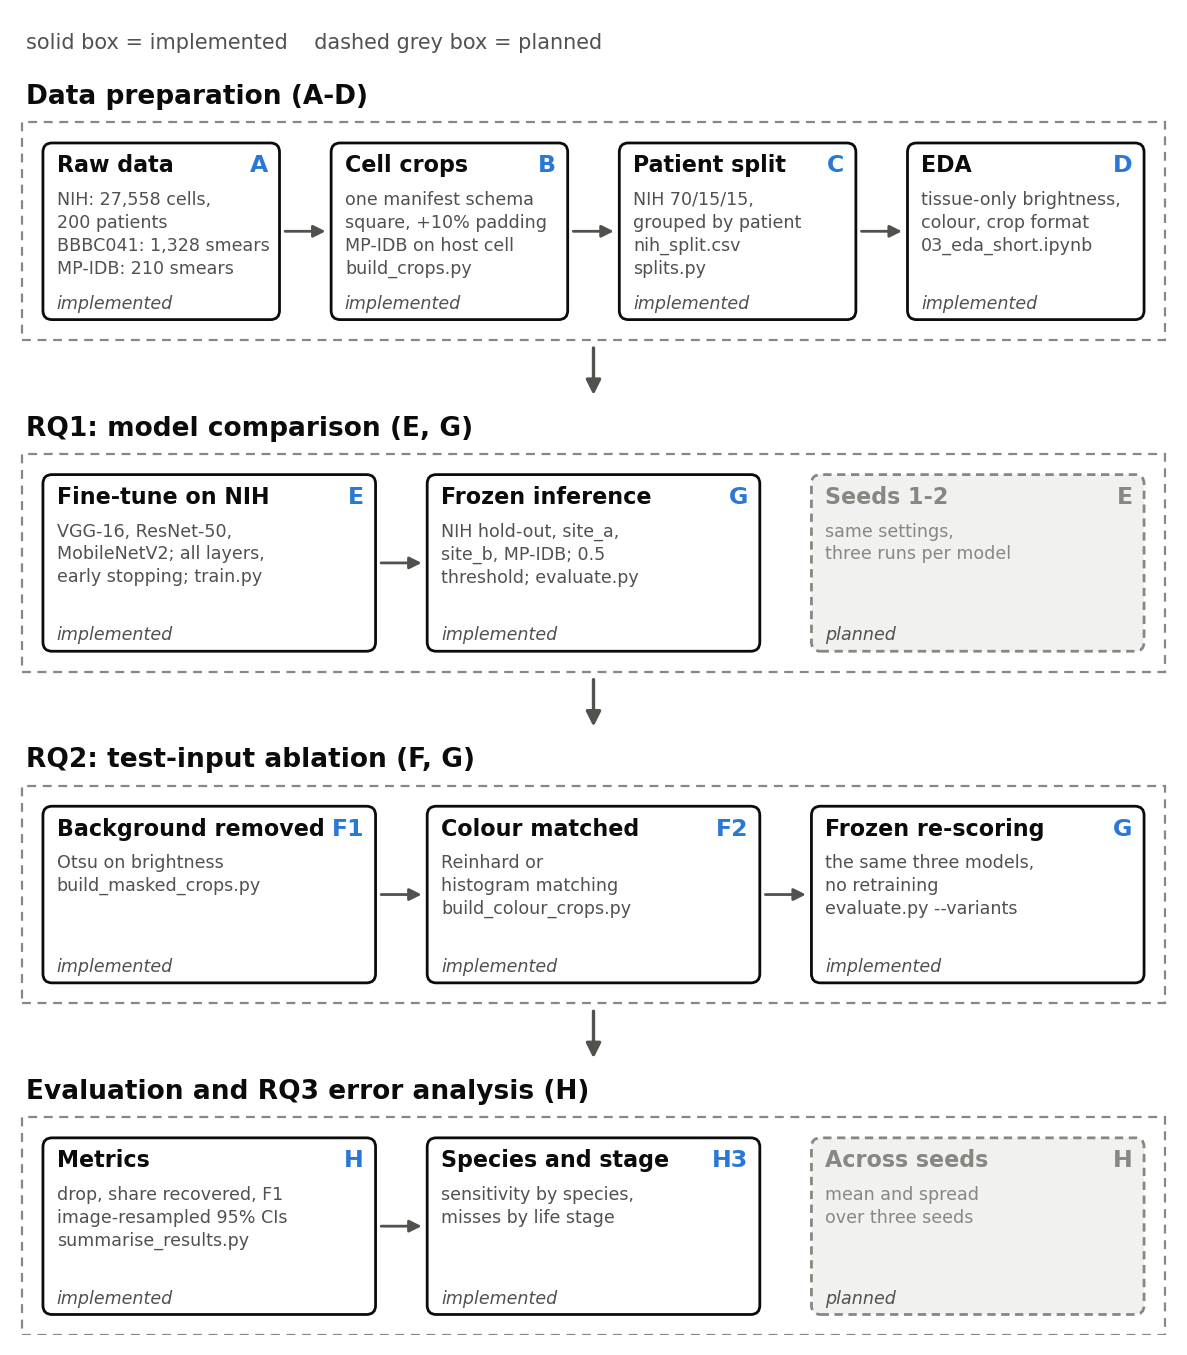
\includegraphics[width=\linewidth,height=0.66\textheight,keepaspectratio]{figures/pipeline_v3.png}
\caption{Pipeline and study design. Each model is trained once on NIH (E), tested frozen on the raw test crops (G, RQ1), tested again on edited copies of the same crops (F, G, RQ2), and its errors are broken down by species and life stage (H3, RQ3). Drawn by \href{https://github.com/noahtjonsk/malaria-cross-dataset/blob/main/scripts/make_mo_figures.py}{\texttt{scripts/\allowbreak{}make\_\allowbreak{}mo\_\allowbreak{}figures.\allowbreak{}py}}.}
\end{figure}

\section{Dataset description and access (stage A)}

\subsection{Sources and access}

All three datasets are public. Neither NIH download has a DOI, so the table cites the dataset paper and the NLM download page. The raw files are not copied into the repository: they sit in the project root, are ignored by git, and are read only through the paths in \href{https://github.com/noahtjonsk/malaria-cross-dataset/blob/main/malaria/paths.py}{\texttt{malaria/\allowbreak{}paths.\allowbreak{}py}}. \texttt{NIH-NLM-ThinBloodSmearsPf} is the release that \texttt{cell\_\allowbreak{}images} was cut from \citep{kassim2021}. 192 of the 200 cell\_\allowbreak{}images patients and 960 of the release's 965 photographs appear in both (\href{https://github.com/noahtjonsk/malaria-cross-dataset/blob/main/outputs/tables/nih_source_overlap.csv}{\texttt{outputs/\allowbreak{}tables/\allowbreak{}nih\_\allowbreak{}source\_\allowbreak{}overlap.\allowbreak{}csv}}, \href{https://github.com/noahtjonsk/malaria-cross-dataset/blob/main/scripts/check_nih_overlap.py}{\texttt{scripts/\allowbreak{}check\_\allowbreak{}nih\_\allowbreak{}overlap.\allowbreak{}py}}), so it is used only to recut NIH cells for the EDA and never as a test set.

{\small
\begin{longtable}{@{}>{\raggedright\arraybackslash\hspace{0pt}}p{90.6pt}>{\raggedright\arraybackslash\hspace{0pt}}p{166.8pt}>{\raggedright\arraybackslash\hspace{0pt}}p{66.6pt}@{}}
\toprule
Dataset & Source and persistent identifier & Role \\
\midrule
\endhead
\bottomrule
\endfoot
\bottomrule
\endlastfoot
NIH cell\_\allowbreak{}images & \citet{rajaraman2018}, \href{https://doi.org/10.7717/peerj.4568}{doi:10.7717/peerj.4568}; download from the \href{https://lhncbc.nlm.nih.gov/LHC-research/LHC-projects/image-processing/malaria-datasheet.html}{NLM malaria datasheet} (downloaded 7 May 2026) & training, validation and hold-out \\*
NIH-NLM-ThinBloodSmearsPf & \citet{kassim2021}, \href{https://doi.org/10.1109/JBHI.2020.3034863}{doi:10.1109/JBHI.2020.3034863}; same NLM page (downloaded 15 Sept 2026) & EDA only (overlaps cell\_\allowbreak{}images) \\*
BBBC041 v1 & \citet{ljosa2012}, \href{https://doi.org/10.1038/nmeth.2083}{doi:10.1038/nmeth.2083}; \citet{hung2017}, \href{https://doi.org/10.1109/CVPRW.2017.112}{doi:10.1109/CVPRW.2017.112}; \href{https://bbbc.broadinstitute.org/BBBC041}{bbbc.broadinstitute.org/BBBC041} (downloaded 7 May 2026) & external test (site\_\allowbreak{}a, site\_\allowbreak{}b) \\*
MP-IDB & \citet{loddo2019}, \href{https://doi.org/10.1007/978-3-030-13835-6_7}{doi:10.1007/978-3-030-13835-6\_\allowbreak{}7}; \href{https://github.com/andrealoddo/MP-IDB-The-Malaria-Parasite-Image-Database-for-Image-Processing-and-Analysis}{GitHub repository} (downloaded 7 May 2026) & external test (four species) \\*
\end{longtable}}
\addtocounter{table}{-1}

\subsection{Quantitative and qualitative description}

The table gives the cell counts at the level the results are reported: by split, acquisition batch, species and life stage. NIH has 27,558 cells from 200 patients and 1,408 photographs. 150 patients contribute parasitised cells and 50 contribute only uninfected cells, and parasitised and uninfected cells are close to 50/50 in every split. BBBC041 is two batches that differ in image size and file format (1,208 images at 1200 $\times$ 1600 in PNG and 120 at 1383 $\times$ 1944 in JPG). The source does not say which batch came from which country, so they are labelled by observable batch, site\_\allowbreak{}a and site\_\allowbreak{}b. Only 2.7\% (site\_\allowbreak{}a) and 5.1\% (site\_\allowbreak{}b) of the cells are parasitised. MP-IDB annotates parasites only, so it has no uninfected cells and specificity cannot be measured on it. \emph{P. falciparum}, the NIH species, accounts for 1,297 of its 1,437 parasites; the other three species together have 140.

{\footnotesize
\begin{longtable}{@{}>{\raggedright\arraybackslash\hspace{0pt}}p{60.4pt}>{\raggedright\arraybackslash\hspace{0pt}}p{106.1pt}>{\raggedleft\arraybackslash}p{31.2pt}>{\raggedleft\arraybackslash}p{53.4pt}>{\raggedleft\arraybackslash}p{49.0pt}@{}}
\toprule
Set & Detail & Images & Parasitised & Uninfected \\
\midrule
\endhead
\bottomrule
\endfoot
\bottomrule
\caption{Cells used in the primary metric, read from \href{https://github.com/noahtjonsk/malaria-cross-dataset/blob/main/data/manifests}{\texttt{data/\allowbreak{}manifests/\allowbreak{}}} through \texttt{malaria.\allowbreak{}data.\allowbreak{}nih\_\allowbreak{}cells} and \texttt{test\_\allowbreak{}cells} (\href{https://github.com/noahtjonsk/malaria-cross-dataset/blob/main/malaria/data.py}{\texttt{malaria/\allowbreak{}data.\allowbreak{}py}}). BBBC041 also has 446 \texttt{difficult} cells and 103 leukocytes, which are excluded (\S{}3.1).}
\endlastfoot
NIH train & 140 patients & 958 & 9,619 & 9,584 \\*
NIH validation & 30 patients & 239 & 2,105 & 2,073 \\*
NIH hold-out & 30 patients & 211 & 2,055 & 2,122 \\*
BBBC041 site\_\allowbreak{}a & ring 353, trophozoite 1,473, schizont 179, gametocyte 144 & 1,208 & 2,149 & 77,420 \\*
BBBC041 site\_\allowbreak{}b & ring 169, trophozoite 111, schizont 11, gametocyte 12 & 120 & 303 & 5,614 \\*
MP-IDB \emph{P. falciparum} & ring 1,230, trophozoite 42, schizont 18, gametocyte 7 & 104 & 1,297 & n/a \\*
MP-IDB other species & \emph{P. malariae} 43, \emph{P. ovale} 33, \emph{P. vivax} 64 & 106 & 140 & n/a \\*
\end{longtable}}

The four sources already look different by eye (Figure 2). NIH cells are segmented and placed on a black background, pink and evenly lit. BBBC041 crops are rectangles cut from the smear: site\_\allowbreak{}a cells are sharp, saturated and often blue-purple, site\_\allowbreak{}b cells are grey and slightly blurred, and both show parts of neighbouring cells. MP-IDB crops are yellow to pink with a visible host cell, and most \emph{P. falciparum} parasites are small rings.

\begin{figure}[H]
\centering
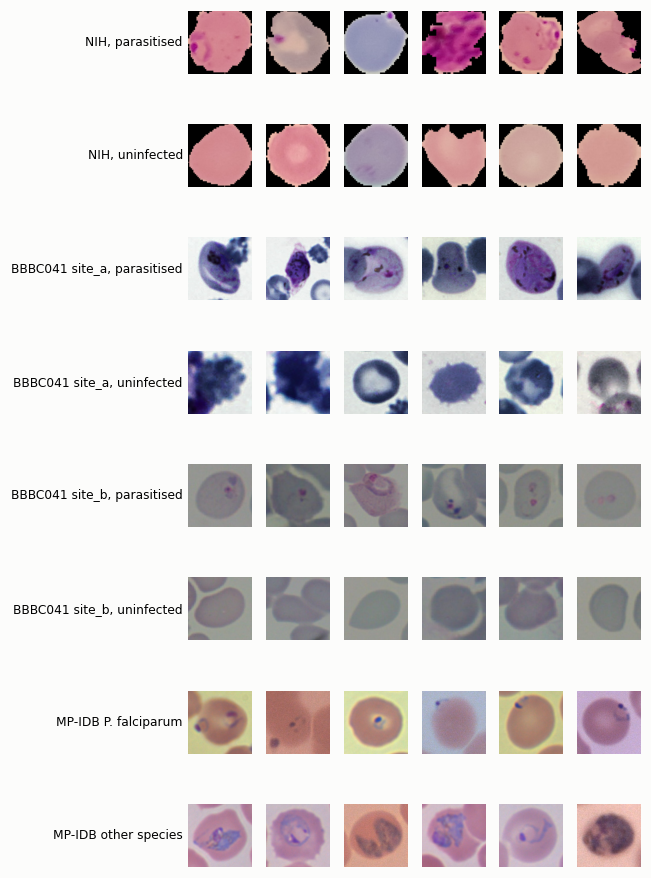
\includegraphics[width=\linewidth,height=0.66\textheight,keepaspectratio]{figures/short_1_example_cells.png}
\caption{Random cells from every test set, as the models see them in RQ1. NIH cells sit on black; the external crops keep their background and parts of neighbouring cells.}
\end{figure}

\subsection{Bias, representativeness and privacy (ELSA)}

\textbf{Privacy.} The images are microscope photographs of blood cells. None of the three releases contains names, ages, sex or clinical data. NIH identifies patients only by a code (\texttt{C\#\#\#}), which this project uses to group the split and for nothing else. No new data are collected.

\textbf{Licences.} BBBC041 is released under CC BY-NC-SA 3.0, which allows non-commercial use and requires derived data to be shared under the same terms. NIH-NLM-ThinBloodSmearsPf may be redistributed as long as NLM's notice is kept and NLM is credited, and the MP-IDB repository is MIT-licensed. The repository therefore holds code, manifests and summary tables only. No image or crop is redistributed, and the Drive copies used for Colab are private and will be deleted after the project.

\textbf{Protected categories.} The data carry no demographic variables, so results cannot be broken down by sex, age or ethnicity. A model could still work worse for some patient groups, and this project would have no way of seeing it; this is reported as a limitation. The subgroups that can be analysed are those in Table 1, which are also the RQ3 subgroups: acquisition batch, species and life stage.

\textbf{Representativeness.} All NIH images come from one hospital, with one staining protocol and one smartphone-on-microscope setup, and show a single species. NIH's 50/50 class balance was made by curation: in the source photographs only 3.3\% of annotated cells are parasitised, close to site\_\allowbreak{}a's 2.7\%. A model tuned to that balance can look better on the hold-out set than it would at clinical prevalence, so sensitivity and specificity are reported separately and accuracy is not. The external sets add a second species (\emph{P. vivax}, BBBC041) and a European reference laboratory (MP-IDB). None of the three has smears from sub-Saharan Africa, where most malaria deaths occur, and the generalisation claims go no further than these three sources.

\textbf{Mitigations (ELSA Part B).} The D5 checklist (deon base items plus project items) is in the ELSA report, \href{https://github.com/noahtjonsk/malaria-cross-dataset/blob/main/docs/elsa_report.md}{\texttt{docs/\allowbreak{}elsa\_\allowbreak{}report.\allowbreak{}md}}, with answers to the panel-review questions. The table repeats its Part B: the mitigation for each item judged critical.

{\small
\begin{longtable}{@{}>{\raggedright\arraybackslash\hspace{0pt}}p{79.7pt}>{\raggedright\arraybackslash\hspace{0pt}}p{256.3pt}@{}}
\toprule
Item & How the project deals with it \\
\midrule
\endhead
\bottomrule
\endfoot
\bottomrule
\caption{ELSA Part B mitigations, copied from the ELSA report, where each row also says where it is implemented.}
\endlastfoot
A.2 Collection bias & Each source is reported as its own domain: site\_\allowbreak{}a and site\_\allowbreak{}b separately, and \emph{P. falciparum} separately from the other species. No pooled score exists that one site could dominate, and the claims cover these three sources only. \\*
A.4 No protected attributes & Disparities by sex, age or ethnicity cannot be measured, and the report says so as a limitation. RQ3 analyses the subgroups that can be measured: acquisition batch, species and life stage. \\*
A.5 Licences & Only code, manifests and summary tables go into the repository. Raw images and crops stay out of git, and so do the Drive copies, which are kept for this non-commercial study only. BBBC041's share-alike term therefore never applies to a redistributed file, and each dataset paper is cited and NLM credited. \\
A.6 Label quality & BBBC041's annotators marked 446 cells as \texttt{difficult}; these and the 103 leukocytes stay in the manifests but are left out of the primary metric. For each of MP-IDB's 210 images, the tracked \texttt{mpidb\_\allowbreak{}stage\_\allowbreak{}audit.\allowbreak{}csv} records how many parasites it holds, how many crops were shipped and where the stage labels came from. NIH labels are used as released. Checking them again is out of scope, which is reported as a limitation. \\
A.7 Overlapping releases & 192 of the 200 cell\_\allowbreak{}images patients and 960 of the release's 965 photographs appear in both NIH releases (\texttt{nih\_\allowbreak{}source\_\allowbreak{}overlap.\allowbreak{}csv}), so NIH-NLM-ThinBloodSmearsPf is never used as a test set. It is used only to recut NIH cells for the EDA, and every recut cell inherits its patient's split (\texttt{inherit\_\allowbreak{}nih\_\allowbreak{}split}), so no patient crosses splits even there. \\
C.2 Prevalence mismatch & The NIH classes are not rebalanced: the model trains at NIH's 50/50 split, and the prevalence mismatch is dealt with at evaluation. Sensitivity and specificity are reported separately because neither depends on prevalence. Accuracy is not reported for BBBC041, and F1 only as a secondary measure. \\
C.6 Patient leakage & The NIH split is by patient, pinned in \texttt{nih\_\allowbreak{}split.\allowbreak{}csv}, and checked before every training run. The overlapping NIH-NLM release is never used as a test set. \\
D.2 Disparate error rates & Sensitivity is compared across species, with an interval on the difference, and across BBBC041 life stages, as share of misses and miss rate. Specificity is compared across the two BBBC041 batches. Every interval comes from resampling source images. \\
D.3 Metric choice & A missed parasite (a patient left untreated) and a false alarm (unnecessary antimalarials) cost different things, so they are reported apart. The threshold is fixed at 0.5 before testing. AUC is only a threshold-free check. \\
D.4 Explainability & Saliency methods such as Grad-CAM were left out of scope in the proposal. RQ2 tests directly what the models depend on: if removing the background or matching the colour changes their decisions, they were using those cues. \\
D.8 Shortcut learning & RQ2's first step puts the test cells into the NIH black-frame format. The share of the drop this recovers shows how much the models relied on the frame instead of the parasite. \\
E.1 Regulation and redress & This is a research prototype, trained and tested on public data and never used on patients. The EU AI Act excludes AI systems developed only for scientific research (Art. 2(6)). A deployed diagnostic version would be a medical device (MDR 2017/745) and a high-risk AI system, requiring clinical validation, which this project does not do. \\
E.5 Untested populations & The three sources are a hospital in Chittagong (NIH), the two acquisition batches of BBBC041 and a laboratory in Lausanne (MP-IDB), and none is from sub-Saharan Africa. Claims are limited to these sources, and each source is reported on its own so that a pooled score cannot hide one of them. The Methodology Overview and the final report both name the missing region as a limitation. \\*
E.6 Automation bias & The models are research prototypes and are never used on patients, as the README, the model information sheet and this report state. Each output is a probability cut at a fixed 0.5 threshold, not a diagnosis, and the seed-0 results show how often that call is wrong on new data: sensitivity on MP-IDB \emph{P. falciparum} is between 28.6\% and 57.4\% across the three models. Clinical use would need a microscopist to confirm every call, plus a separate clinical validation. \\*
\end{longtable}}

\section{Dataset cleaning, preprocessing and splitting (stages B and C)}

\subsection{Cropping, manifests and exclusions (stage B)}

\textbf{Scripts:} \href{https://github.com/noahtjonsk/malaria-cross-dataset/blob/main/scripts/build_crops.py}{\texttt{scripts/\allowbreak{}build\_\allowbreak{}crops.\allowbreak{}py}}, \href{https://github.com/noahtjonsk/malaria-cross-dataset/blob/main/malaria/manifests.py}{\texttt{malaria/\allowbreak{}manifests.\allowbreak{}py}}, \href{https://github.com/noahtjonsk/malaria-cross-dataset/blob/main/malaria/crops.py}{\texttt{malaria/\allowbreak{}crops.\allowbreak{}py}}, \href{https://github.com/noahtjonsk/malaria-cross-dataset/blob/main/malaria/background.py}{\texttt{malaria/\allowbreak{}background.\allowbreak{}py}}

Every cell, from any dataset, becomes a row in a manifest with one shared schema (\texttt{manifests.\allowbreak{}COLUMNS}): dataset, split, cell ID, crop path, binary label, evaluation group, stage, species, patient, source image and crop box. Later stages read cells only through these tables. The steps are applied in this order:

{\small
\begin{longtable}{@{}>{\raggedright\arraybackslash\hspace{0pt}}p{25.5pt}>{\raggedright\arraybackslash\hspace{0pt}}p{185.5pt}>{\raggedright\arraybackslash\hspace{0pt}}p{113.0pt}@{}}
\toprule
Step & Operation & Justification \\
\midrule
\endhead
\bottomrule
\endfoot
\bottomrule
\endlastfoot
1 & Build one manifest per dataset (\texttt{build\_\allowbreak{}nih\_\allowbreak{}manifest}, \texttt{build\_\allowbreak{}bbbc041\_\allowbreak{}manifest}, \texttt{build\_\allowbreak{}mpidb\_\allowbreak{}wholecell\_\allowbreak{}manifest}) & One schema means every later stage treats the datasets the same way. \\*
2 & Cut BBBC041 cells with one rule (\texttt{crops.\allowbreak{}square\_\allowbreak{}padded\_\allowbreak{}box}): a square around the annotated box, padded by 10\%, clipped and flagged where it meets the image border & A square crop matches the square NIH input; the padding keeps the whole cell edge in view. \\*
3 & Recentre MP-IDB crops on the red cell that holds each parasite (\texttt{background.\allowbreak{}host\_\allowbreak{}cell\_\allowbreak{}box}, \texttt{build\_\allowbreak{}crops.\allowbreak{}py --mpidb-wholecell}). The host cell was found for 1,091 of the 1,437 parasites; the other 346 (340 \emph{P. falciparum}: 338 in cell clumps and 2 missed; 6 \emph{P. malariae}) fall back to a cell-sized square centred on the parasite (\href{https://github.com/noahtjonsk/malaria-cross-dataset/blob/main/outputs/tables/mpidb_wholecell_framing.csv}{\texttt{mpidb\_\allowbreak{}wholecell\_\allowbreak{}framing.\allowbreak{}csv}}) & MP-IDB annotates parasites, not cells, and NIH crops show a whole cell. The shipped close-ups cut off the cell edge and mix masked and unmasked formats by species. \\
4 & Exclude BBBC041 \texttt{difficult} cells (446) and leukocytes (103). They stay in the manifest with \texttt{eval\_\allowbreak{}group} set to \texttt{excluded\_\allowbreak{}*}, and \texttt{data.\allowbreak{}test\_\allowbreak{}cells} returns only \texttt{primary} rows & \texttt{difficult} cells are ambiguous by the annotators' own label, and leukocytes are a class the model never saw (the NIH negative class is uninfected red cells). \\
5 & Never use NIH-NLM-ThinBloodSmearsPf or the MP-IDB parasite close-ups (\texttt{mpidb}) as evaluation sets & The first overlaps cell\_\allowbreak{}images (\S{}2.1); every RQ evaluates whole cells. \\*
6 & Check for missing values & None among the primary cells: each has a path, a label and a source image, and \texttt{CellDataset} raises an error on an unlabelled row. \\*
\end{longtable}}
\addtocounter{table}{-1}

Output: \texttt{data/\allowbreak{}manifests/\allowbreak{}*\_\allowbreak{}cells.\allowbreak{}csv} (rebuilt deterministically, so gitignored) and the crops under \texttt{data/\allowbreak{}crops/\allowbreak{}}, saved as PNG by dataset, split and class so they can be browsed in a file explorer (see the table in \href{https://github.com/noahtjonsk/malaria-cross-dataset/blob/main/README.md}{\texttt{README.\allowbreak{}md}}). The reframing keeps every MP-IDB parasite, stage label and cell ID, which the build asserts.

\subsection{Patient-grouped split (stage C)}

\textbf{Script:} \href{https://github.com/noahtjonsk/malaria-cross-dataset/blob/main/malaria/splits.py}{\texttt{malaria/\allowbreak{}splits.\allowbreak{}py}}; pinned output \href{https://github.com/noahtjonsk/malaria-cross-dataset/blob/main/data/manifests/nih_split.csv}{\texttt{data/\allowbreak{}manifests/\allowbreak{}nih\_\allowbreak{}split.\allowbreak{}csv}}

NIH is split 70/15/15 by patient (\texttt{splits.\allowbreak{}patient\_\allowbreak{}grouped\_\allowbreak{}split}, seed 42). Patients are assigned greedily, largest first, to whichever split is furthest below its target number of cells, so no patient is split. The assignment does not target class balance, but every split stays close to 50/50 (Table 3). The split was computed once and written to the tracked \texttt{nih\_\allowbreak{}split.\allowbreak{}csv}, so all three architectures train on the same rows. The external test sets are kept whole and never split: the models do not see them until stage G.

{\footnotesize
\begin{longtable}{@{}>{\raggedright\arraybackslash\hspace{0pt}}p{169.7pt}>{\raggedleft\arraybackslash}p{36.3pt}>{\raggedleft\arraybackslash}p{58.6pt}>{\raggedleft\arraybackslash}p{47.4pt}@{}}
\toprule
 & Train & Validation & Hold-out \\
\midrule
\endhead
\bottomrule
\endfoot
\bottomrule
\caption{The three NIH splits have similar shares of uninfected-only patients and almost the same class balance.}
\endlastfoot
Cells & 19,203 & 4,178 & 4,177 \\*
Patients & 140 & 30 & 30 \\*
of which only uninfected cells & 36 & 7 & 7 \\*
Photographs & 958 & 239 & 211 \\*
\% parasitised & 50.1 & 50.4 & 49.2 \\*
\end{longtable}}

\subsection{Data leakage}

\citet{kapoor2023} define leakage as a spurious relationship between inputs and target that comes from the data collection, sampling or preprocessing. The table lists each route that applies here and how it is closed. The model information sheet in Appendix B summarises the training population and the external evaluation.

{\small
\begin{longtable}{@{}>{\raggedright\arraybackslash\hspace{0pt}}p{83.6pt}>{\raggedright\arraybackslash\hspace{0pt}}p{121.1pt}>{\raggedright\arraybackslash\hspace{0pt}}p{119.3pt}@{}}
\toprule
Leakage route & Risk here & Prevention \\
\midrule
\endhead
\bottomrule
\endfoot
\bottomrule
\endlastfoot
No clean train/test separation & cells of one patient share a slide, stain and lighting & split by patient; \texttt{check\_\allowbreak{}no\_\allowbreak{}patient\_\allowbreak{}leakage} runs before every training job \\*
Duplicates across splits & the same cell saved twice & exact hashes: none; perceptual-hash matches join different patients (EDA section B) \\*
Test data in preprocessing & colour reference or threshold fitted on test cells & colour reference from NIH train only; threshold fixed at 0.5 before testing \\*
Model selection on test data & choosing epochs, methods or thresholds by test score & early stopping on NIH validation only; both colour methods reported \\*
Overlapping releases & NIH-NLM-ThinBloodSmearsPf photographs the same patients & never used as a test set; recut cells inherit their patient's split (\texttt{inherit\_\allowbreak{}nih\_\allowbreak{}split}) \\*
\end{longtable}}
\addtocounter{table}{-1}

\subsection{Data-quality issues and continuous-analysis checks}

Table 4 lists every oddity found while preparing the data and what was done about it.

{\small
\begin{longtable}{@{}>{\raggedright\arraybackslash\hspace{0pt}}p{69.8pt}>{\raggedright\arraybackslash\hspace{0pt}}p{135.5pt}>{\raggedright\arraybackslash\hspace{0pt}}p{118.7pt}@{}}
\toprule
Issue & Finding & Status \\
\midrule
\endhead
\bottomrule
\endfoot
\bottomrule
\caption{Data-quality issues found during preparation and their status.}
\endlastfoot
NIH cells on black padding & The median NIH crop is 26\% black padding; no external crop has any. & Kept as the training format. The EDA measures tissue pixels only (\S{}4), and RQ2 step F1 gives test cells the same frame (\S{}5.2). \\*
MP-IDB has no uninfected cells & Only parasites are annotated. & Specificity, AUC, precision and F1 are measured on NIH and BBBC041 only. \\*
MP-IDB close-ups & The shipped crops show the parasite, cut off the cell edge, and are masked for some species and not for others. & Fixed: every parasite is reframed on its host red cell (\S{}3.1, step 3). \\
Host cell not found & 346 MP-IDB parasites (340 \emph{P. falciparum}, 6 \emph{P. malariae}) get a cell-sized square instead. & Kept; RQ3 is also reported without them (\texttt{rq3\_\allowbreak{}<model>\_\allowbreak{}s0\_\allowbreak{}without\_\allowbreak{}fallback.\allowbreak{}csv}). \\
Mask centre on background & For 1,029 of the 86,035 BBBC041 crops (1,022 of them primary cells), Otsu found no cell under the crop centre and kept the nearest region, which may be a neighbour. & Kept; RQ2 is also reported without these cells (\texttt{rq2\_\allowbreak{}<model>\_\allowbreak{}s0\_\allowbreak{}without\_\allowbreak{}nearest.\allowbreak{}csv}). \\
Ambiguous and out-of-scope cells & BBBC041 has 446 \texttt{difficult} cells and 103 leukocytes. & Excluded from the primary metric, kept in the manifests (\S{}3.1, step 4). \\
Overlapping NIH releases & 192 of 200 patients and 960 of 965 photographs are shared. & The NIH-NLM release is never a test set (\S{}3.3). \\
Errors found in code review & Reinhard transfer used a spread pooled over many cells, histogram matching broke ties toward the dark end, and the NIH bootstrap resampled photographs instead of patients. & Fixed before the results in \S{}5.6; VGG-16 was re-scored on the corrected crops. \\*
Missing values & None among the primary cells. & \texttt{CellDataset} raises an error on an unlabelled row. \\*
\end{longtable}}

There is no separate test suite. The checks run inside the pipeline \citep{beaulieujones2017}, so a run that breaks an assumption stops with an error instead of producing numbers. Among them: the NIH split sizes must equal the pinned 19,203 / 4,178 / 4,177; no patient may appear in two splits; every model parameter must be trainable; the reframing must keep every MP-IDB parasite; a perfect predictor must score 1 on every metric in \texttt{python -m malaria.\allowbreak{}metrics}; and models are compared only if they were scored on the same manifests, crop contents and cells. The full list is in Appendix C.

The build scripts must run in a fixed order, because each reads the output of the previous one: \texttt{build\_\allowbreak{}crops.\allowbreak{}py} (manifests and crops), then \texttt{compute\_\allowbreak{}stats.\allowbreak{}py} (EDA statistics), then \texttt{build\_\allowbreak{}masked\_\allowbreak{}crops.\allowbreak{}py} and \texttt{build\_\allowbreak{}colour\_\allowbreak{}crops.\allowbreak{}py} (RQ2 inputs), and only then training and evaluation (\S{}6).

\section{Exploratory data analysis (stage D)}

The EDA (\href{https://github.com/noahtjonsk/malaria-cross-dataset/blob/main/notebooks/03_eda_short.ipynb}{\texttt{notebooks/\allowbreak{}03\_\allowbreak{}eda\_\allowbreak{}short.\allowbreak{}ipynb}}, full record in \href{https://github.com/noahtjonsk/malaria-cross-dataset/blob/main/notebooks/01_eda.ipynb}{\texttt{01\_\allowbreak{}eda.\allowbreak{}ipynb}}) measured every cell on tissue pixels only, because a quarter of each NIH crop is black padding that would otherwise dilute brightness and colour averages (\href{https://github.com/noahtjonsk/malaria-cross-dataset/blob/main/malaria/imagestats.py}{\texttt{malaria/\allowbreak{}imagestats.\allowbreak{}py}}, \href{https://github.com/noahtjonsk/malaria-cross-dataset/blob/main/scripts/compute_stats.py}{\texttt{scripts/\allowbreak{}compute\_\allowbreak{}stats.\allowbreak{}py}}). Differences are reported as a rank-based separation between 0 (identical distributions) and 1 (no overlap), computed in \texttt{imagestats.\allowbreak{}separation}. Three findings decided the method.

{\small
\begin{longtable}{@{}>{\raggedright\arraybackslash\hspace{0pt}}p{68.2pt}>{\raggedright\arraybackslash\hspace{0pt}}p{172.4pt}>{\raggedright\arraybackslash\hspace{0pt}}p{83.4pt}@{}}
\toprule
Finding & Evidence & Consequence \\
\midrule
\endhead
\bottomrule
\endfoot
\bottomrule
\caption{The three EDA findings that shaped the method.}
\endlastfoot
Crop format is the largest difference (Figure 3) & The median NIH crop is 26\% black padding, and no external crop has any. Separation on the fraction of black pixels is 1.00 against every test set. & RQ2 step F1 removes the background of the test crops. \\*
Stain colour differs, in a different direction per test set (Figure 4) & After Giemsa colour deconvolution, BBBC041 cells absorb three to four times as much methyl blue as NIH cells (median 0.065 to 0.090 against 0.022). On the red-minus-blue axis NIH sits close to MP-IDB \emph{P. falciparum}, while BBBC041 sits at or below zero. A hue and saturation shift toward NIH moves methyl blue further away (separation 0.88 against 0.72); Reinhard transfer or histogram matching brings both stain channels close to NIH (\href{https://github.com/noahtjonsk/malaria-cross-dataset/blob/main/outputs/tables/colour_transform_effect.csv}{\texttt{colour\_\allowbreak{}transform\_\allowbreak{}effect.\allowbreak{}csv}}). & RQ2 step F2 uses Reinhard transfer and histogram matching, not an HSV shift. \\*
Sharpness differs in both directions & site\_\allowbreak{}a and \emph{P. malariae} are sharper than NIH; site\_\allowbreak{}b, \emph{P. ovale} and \emph{P. vivax} are blurrier. & A blur sweep cannot reproduce the shift, so the proposal's blur, noise and contrast experiments were dropped from RQ2. \\*
\end{longtable}}

\begin{figure}[H]
\centering
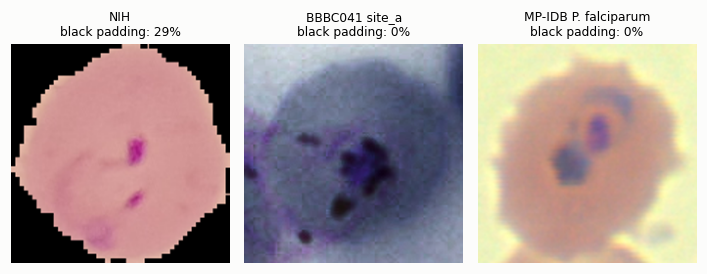
\includegraphics[width=\linewidth,height=0.66\textheight,keepaspectratio]{figures/short_3_crop_format.png}
\caption{Crop format. NIH cells are segmented and placed on black; the external crops are rectangles cut from the smear.}
\end{figure}

\begin{figure}[H]
\centering
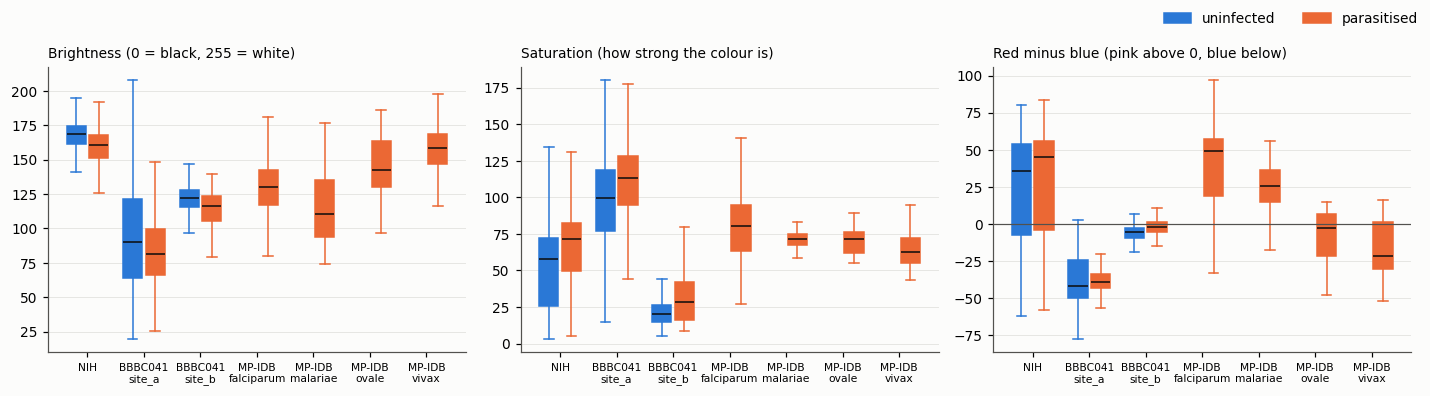
\includegraphics[width=\linewidth,height=0.66\textheight,keepaspectratio]{figures/short_4_brightness_colour.png}
\caption{Tissue brightness, saturation and red minus blue per test set and class (boxes: quartiles; whiskers: 5th to 95th percentile).}
\end{figure}

Single cells were looked at as well as distributions. Figure 2 shows random cells per set and class, and the full EDA record adds contact sheets and the smallest crops of each set, which were checked by eye for cut-off cells.

\section{Models and evaluation (stages E to H)}

\subsection{Model arms and baseline protocol (stage E)}

\textbf{Scripts:} \href{https://github.com/noahtjonsk/malaria-cross-dataset/blob/main/malaria/models.py}{\texttt{malaria/\allowbreak{}models.\allowbreak{}py}}, \href{https://github.com/noahtjonsk/malaria-cross-dataset/blob/main/malaria/data.py}{\texttt{malaria/\allowbreak{}data.\allowbreak{}py}}, \href{https://github.com/noahtjonsk/malaria-cross-dataset/blob/main/scripts/train.py}{\texttt{scripts/\allowbreak{}train.\allowbreak{}py}}, \href{https://github.com/noahtjonsk/malaria-cross-dataset/blob/main/notebooks/10_train_colab.ipynb}{\texttt{notebooks/\allowbreak{}10\_\allowbreak{}train\_\allowbreak{}colab.\allowbreak{}ipynb}}

RQ1 compares one lightweight and two heavy architectures, all built by \texttt{models.\allowbreak{}build\_\allowbreak{}model} from torchvision's ImageNet weights \citep{russakovsky2015}, with the 1,000-class head replaced by a single output. They are the three networks named in the proposal, and they span a sixty-fold range in size while sharing an input size and a pretraining dataset.

{\footnotesize
\begin{longtable}{@{}>{\raggedright\arraybackslash\hspace{0pt}}p{20.4pt}>{\raggedright\arraybackslash\hspace{0pt}}p{89.2pt}>{\raggedleft\arraybackslash}p{72.6pt}>{\raggedright\arraybackslash\hspace{0pt}}p{129.8pt}@{}}
\toprule
Arm & Model & Parameters (with new head) & Rationale \\
\midrule
\endhead
\bottomrule
\endfoot
\bottomrule
\endlastfoot
E1 & VGG-16 \citep{simonyan2015} & 134.3 M & Plain stacked convolutions; the oldest and largest network \\*
E2 & ResNet-50 \citep{he2016} & 23.5 M & Residual network; the standard heavy contender \\*
E3 & \mbox{MobileNetV2} \citep{sandler2018} & 2.2 M & The lighter architecture RQ1 asks about \\*
\end{longtable}}
\addtocounter{table}{-1}

Following the literature review (\S{}2.3), the baseline is the patient-grouped protocol of \citet{hou2026} applied to all three architectures, not one model.

\begin{itemize}
\item \emph{Architecture.} torchvision weights \texttt{IMAGENET1K\_\allowbreak{}V1} for all three, so the pretraining recipe is the same generation. The last layer becomes a single-output linear layer whose output is the logit for \emph{parasitised}: \texttt{classifier[6]} in VGG-16, \texttt{fc} in ResNet-50, \texttt{classifier[1]} in \mbox{MobileNetV2}.
\item \emph{Fine-tuning.} Every parameter is trained (VGG-16 134,264,641; ResNet-50 23,510,081; \mbox{MobileNetV2} 2,225,153); no layer is frozen, and \texttt{check\_\allowbreak{}all\_\allowbreak{}trainable} asserts this before and after training.
\item \emph{Input.} Each crop is padded to a square with black, resized to 224 $\times$ 224 and normalised with the ImageNet channel means and standard deviations (\texttt{data.\allowbreak{}pad\_\allowbreak{}to\_\allowbreak{}square}, \texttt{data.\allowbreak{}load\_\allowbreak{}input}).
\item \emph{Training.} Binary cross-entropy on the logit, Adam \citep{kingma2015}, mixed precision on the GPU.
\item \emph{Output.} \texttt{models/\allowbreak{}<model>\_\allowbreak{}s<seed>.\allowbreak{}pt}, a per-epoch log (\texttt{outputs/\allowbreak{}tables/\allowbreak{}<model>\_\allowbreak{}s0\_\allowbreak{}training\_\allowbreak{}log.\allowbreak{}json}) and a resumable checkpoint written after every epoch. A resumed run must have the settings it started with, and keeps the commit it started at.
\item \emph{Where it runs.} A Colab T4 GPU through \texttt{notebooks/\allowbreak{}10\_\allowbreak{}train\_\allowbreak{}colab.\allowbreak{}ipynb}, which unpacks the archive built by \href{https://github.com/noahtjonsk/malaria-cross-dataset/blob/main/scripts/pack_for_colab.py}{\texttt{scripts/\allowbreak{}pack\_\allowbreak{}for\_\allowbreak{}colab.\allowbreak{}py}}. On the laptop, \texttt{train.\allowbreak{}py --smoke} checks the same code on 64 cells.
\end{itemize}

\textbf{Class balance and resampling.} NIH training cells are 50.1\% parasitised, so there is no undersampling, oversampling or loss reweighting. The imbalance that matters is in the test sets (2.7 to 5.1\% parasitised on BBBC041), and it is handled by reporting sensitivity and specificity separately, since neither depends on prevalence.

\subsection{RQ2 test inputs (stage F)}

\textbf{Scripts:} \href{https://github.com/noahtjonsk/malaria-cross-dataset/blob/main/scripts/build_masked_crops.py}{\texttt{scripts/\allowbreak{}build\_\allowbreak{}masked\_\allowbreak{}crops.\allowbreak{}py}}, \href{https://github.com/noahtjonsk/malaria-cross-dataset/blob/main/scripts/build_colour_crops.py}{\texttt{scripts/\allowbreak{}build\_\allowbreak{}colour\_\allowbreak{}crops.\allowbreak{}py}}, \href{https://github.com/noahtjonsk/malaria-cross-dataset/blob/main/malaria/colour.py}{\texttt{malaria/\allowbreak{}colour.\allowbreak{}py}}

RQ2 changes only the test crops; the trained models stay fixed. The two steps follow from the EDA (\S{}4).

{\small
\begin{longtable}{@{}>{\raggedright\arraybackslash\hspace{0pt}}p{25.5pt}>{\raggedright\arraybackslash\hspace{0pt}}p{160.2pt}>{\raggedright\arraybackslash\hspace{0pt}}p{138.3pt}@{}}
\toprule
Step & Operation & Justification \\
\midrule
\endhead
\bottomrule
\endfoot
\bottomrule
\endlastfoot
F0 & Raw crops from \S{}3.1, background kept & The RQ1 input. \\*
F1 & Threshold each test crop on brightness with Otsu's method \citep{otsu1979}. Keep the connected region under the crop centre, or the nearest one when the centre falls on background (1,029 of 86,035 BBBC041 crops); for MP-IDB keep the region that holds the annotated parasite and add the parasite pixels back. Set everything else to black and cut the result to the square around the kept cell. All 87,472 test crops were processed and no mask came back empty & This is how cell\_\allowbreak{}images crops are cut. Otsu reached a median Dice of 0.90 against the NIH hand-drawn outlines, while rembg U\textsuperscript{2}-Net found no cell in 21\% of NIH crops (\href{https://github.com/noahtjonsk/malaria-cross-dataset/blob/main/outputs/tables/background_method_summary.csv}{\texttt{background\_\allowbreak{}method\_\allowbreak{}summary.\allowbreak{}csv}}). Adding the parasite back means no parasite is removed (median retention before that step 0.98 to 1.00). \\*
F2a & Reinhard transfer \citep{reinhard2001}: match the mean and standard deviation of each Lab channel to the average per-cell mean and standard deviation of NIH cells (\texttt{colour.\allowbreak{}reinhard}) & It rescales each cell's own spread; a spread pooled over many cells would add the differences \emph{between} NIH cells and inflate every test cell's contrast. \\*
F2b & Histogram matching: map each RGB channel's quantiles to the pooled NIH quantiles (\texttt{colour.\allowbreak{}match\_\allowbreak{}to\_\allowbreak{}reference}) & A second, non-parametric way to reach the NIH colour distribution. \\*
\end{longtable}}
\addtocounter{table}{-1}

Both F2 methods use tissue pixels only and start from the F1 crops. The NIH reference comes from 1,000 randomly drawn \emph{training} cells (seed 0), saved to \href{https://github.com/noahtjonsk/malaria-cross-dataset/blob/main/outputs/tables/colour_reference.json}{\texttt{outputs/\allowbreak{}tables/\allowbreak{}colour\_\allowbreak{}reference.\allowbreak{}json}}, so no hold-out cell affects the test inputs. Both methods are reported; neither is chosen by its test score.

\begin{figure}[H]
\centering
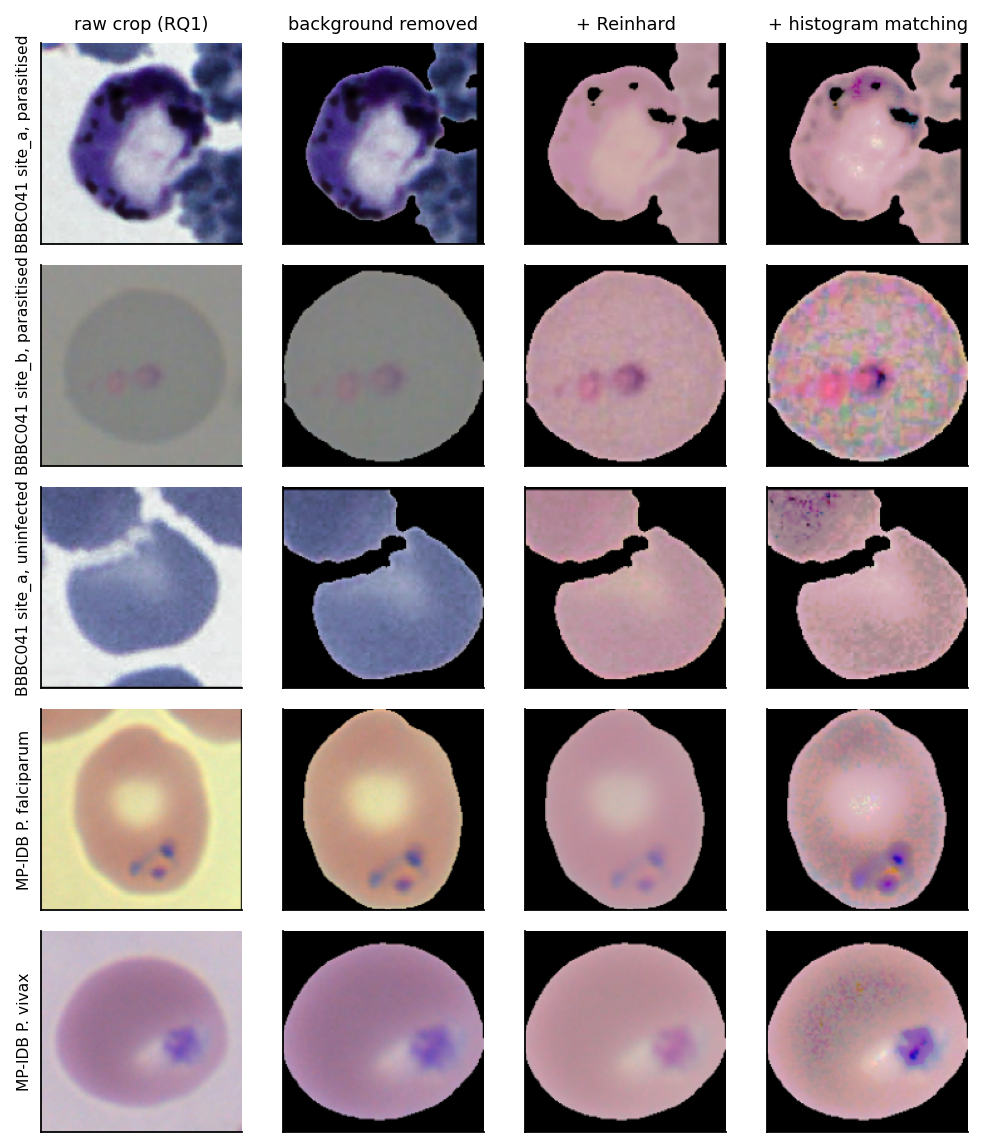
\includegraphics[width=\linewidth,height=0.66\textheight,keepaspectratio]{figures/rq2_variants.png}
\caption{The same test cells as RQ1 and RQ2 see them. Three known artefacts are visible. On BBBC041, Otsu keeps a touching neighbour together with the cell (rows 1 and 3). Very dark site\_\allowbreak{}a pixels fall below the black level and are treated as padding (row 1). Histogram matching stretches the small colour spread of the grey site\_\allowbreak{}b cells and amplifies their noise (row 2).}
\end{figure}

\subsection{Hyperparameters}

All values are fixed in advance (\texttt{SETTINGS} in \texttt{train.\allowbreak{}py}, \texttt{data.\allowbreak{}py}, \texttt{models.\allowbreak{}py}) and are the same for the three arms; \texttt{--resume} refuses a run whose settings changed. \emph{Importance} says how much changing the value would be expected to change the RQ results.

{\footnotesize
\begin{longtable}{@{}>{\raggedright\arraybackslash\hspace{0pt}}p{70.2pt}>{\raggedright\arraybackslash\hspace{0pt}}p{93.5pt}>{\raggedright\arraybackslash\hspace{0pt}}p{50.6pt}>{\raggedright\arraybackslash\hspace{0pt}}p{97.6pt}@{}}
\toprule
Hyperparameter & Value & Importance & Why this value \\
\midrule
\endhead
\bottomrule
\endfoot
\bottomrule
\caption{Every hyperparameter, its value and its expected importance.}
\endlastfoot
Learning rate & 1 $\times$ 10\textsuperscript{\textminus{}4} & high & Controls how far the pretrained weights move. \citet{loddo2022} fine-tuned the same three networks on NIH at this rate; in their tests, smaller rates learned too slowly and larger ones did not converge. \citet{rajaraman2019} also trained every layer at this low rate. \\*
Epochs and early stopping & at most 20; stop when NIH validation loss has not improved for 3 epochs; keep the best-validation weights & high & Decides how closely each model fits the NIH training patients. Early stopping replaces the fixed ten epochs of \citet{loddo2022}, so a model cannot keep training after validation loss stops improving. All three models stopped early (Figure 6). \\*
Decision threshold & 0.5 (\texttt{metrics.\allowbreak{}THRESHOLD}), fixed before any test set was seen & high & Sets the balance between sensitivity and specificity, the reported measures. At seed 0 the architectures differ mostly in where their scores fall relative to it (\S{}5.6). \\
Pretrained weights and trained layers & torchvision \texttt{IMAGENET1K\_\allowbreak{}V1}; every layer trained & high & Stain and cell texture are far from ImageNet photographs, so the early layers need to adapt too; a frozen network with a new head \citep{rajaraman2018} can only reweight ImageNet features. \\
Batch size & 32 & medium & Affects gradient noise and memory. 32 follows \citet{loddo2022} and fits VGG-16 on a T4. \\
Augmentation & horizontal and vertical flips, rotation by multiples of 90\textdegree{} (\texttt{data.\allowbreak{}augment}); no colour jitter & medium & A cell turned upside down is still the same cell, and these flips and rotations change neither its colour nor the black frame. Colour jitter is left out on purpose. A model trained to ignore colour would leave less for RQ2's colour step to recover, by an amount that depends on an arbitrary jitter strength. \citet{hou2026} trained with colour jitter and still saw specificity fall to 18.0\% on BBBC041. \\
Input & 224 $\times$ 224, black padding to square, ImageNet mean and standard deviation & medium & Matches the pretrained weights; black padding matches how NIH crops are stored. \\
Optimiser & Adam, betas (0.9, 0.999), weight decay 0 & low & PyTorch defaults, as in \citet{loddo2022}; not varied. \\
Loss & \texttt{BCEWithLogitsLoss}, no class weights & low & The training data are 50.1\% parasitised, so there is nothing to reweight. \\
Dropout & torchvision defaults: VGG-16 0.5, \mbox{MobileNetV2} 0.2, ResNet-50 none & low & Each network is used as published. \\
Mixed precision & on the GPU only & low & Speeds up training; the model and loss are unchanged. \\*
Seeds & training 0 (0 to 2 planned); split 42; colour reference 0; bootstrap 0 & low per value & One seed fixes one run; the final results report the spread over three training seeds per architecture. \\*
\end{longtable}}

No grid search or Optuna is used. Tuning each architecture separately would turn part of the RQ1 comparison into a comparison of tuning budgets, and a free Colab GPU cannot run a search over three large networks. Only the seed varies, so each final result is a spread over three runs.

\subsection{Fair model comparison}

The following are held constant across the three arms and across the RQ2 variants:

\begin{itemize}
\item the NIH train, validation and hold-out rows in \texttt{nih\_\allowbreak{}split.\allowbreak{}csv};
\item the input pipeline (black padding to square, 224 px, ImageNet normalisation) and augmentation;
\item the optimiser, learning rate, batch size and stopping rule;
\item the test cells: the same primary rows of NIH hold-out, BBBC041 site\_\allowbreak{}a and site\_\allowbreak{}b, MP-IDB \emph{P. falciparum} and other species;
\item the decision threshold of 0.5, fixed before any test set was seen;
\item the metric code and the bootstrap: each set's resamples are keyed by its name, so every model and variant is resampled on the same NIH patients and test photographs;
\item the code commit and the inputs, checked: \texttt{run.\allowbreak{}json} records, per prediction file, the checkpoint, the manifest hashes and a digest of the crops read, and \texttt{compare\_\allowbreak{}models.\allowbreak{}py} refuses models whose inputs differ.
\end{itemize}

Between arms only the architecture changes, and between RQ2 variants only the test input, so a difference in drop can be traced to one or the other.

\subsection{Evaluation strategy (stages G and H)}

\textbf{Scripts:} \href{https://github.com/noahtjonsk/malaria-cross-dataset/blob/main/scripts/evaluate.py}{\texttt{scripts/\allowbreak{}evaluate.\allowbreak{}py}}, \href{https://github.com/noahtjonsk/malaria-cross-dataset/blob/main/malaria/metrics.py}{\texttt{malaria/\allowbreak{}metrics.\allowbreak{}py}}, \href{https://github.com/noahtjonsk/malaria-cross-dataset/blob/main/scripts/summarise_results.py}{\texttt{scripts/\allowbreak{}summarise\_\allowbreak{}results.\allowbreak{}py}}, \href{https://github.com/noahtjonsk/malaria-cross-dataset/blob/main/scripts/compare_models.py}{\texttt{scripts/\allowbreak{}compare\_\allowbreak{}models.\allowbreak{}py}}

\textbf{Metrics.} All definitions follow Table 2 of the literature review. The task is binary classification with parasitised as the positive class. \emph{Sensitivity} is the share of parasitised cells called parasitised, and \emph{specificity} the share of uninfected cells called uninfected. Specificity is measured on NIH and BBBC041 only, since MP-IDB has no uninfected cells. AUC is a threshold-free check on NIH and BBBC041. The \emph{drop} is the NIH hold-out value minus the test-set value, in percentage points, per model and test set (\texttt{metrics.\allowbreak{}drop\_\allowbreak{}pp}).

\textbf{Why not accuracy or F1 as the main metric.} At 2.7\% prevalence, a model that calls every BBBC041 cell uninfected scores 97.3\% accuracy. F1 combines sensitivity with precision, and precision falls with prevalence even when the model stays the same: \citet{hou2026} show that a single operating point gives a precision of 15 to 27\% below 1\% prevalence and 66 to 90\% at 5 to 20\%. F1 is reported as a secondary measure on NIH and BBBC041 only (\texttt{metrics.\allowbreak{}precision\_\allowbreak{}f1}), with precision and each set's prevalence next to it. No drop in F1 is computed, because the NIH hold-out set is 49.2\% parasitised and site\_\allowbreak{}a 2.7\%. On MP-IDB, precision is 100\% by construction and F1 would only repeat sensitivity. AUC has its own blind spot: a high AUC can sit alongside an unusable operating point, as when \citet{zhao2020} report an AUC of 0.945 on BBBC041 while \citet{hou2026} found 18.0\% specificity at their threshold.

\textbf{Uncertainty.} Every value has a 95\% percentile interval from a bootstrap that resamples \emph{source images}, not cells (\texttt{metrics.\allowbreak{}bootstrap}, 2,000 resamples for every metric). Cells cut from one photograph share its stain, focus and lighting, so treating them as independent would make the intervals too narrow. The NIH hold-out set is resampled one level higher, by \emph{patient} (30 patients, \texttt{metrics.\allowbreak{}reference\_\allowbreak{}draws}), since a patient's photographs come from one slide. The test sets have no patient identifiers, so they are resampled by photograph. The interval for a drop comes from resampling the NIH hold-out set and the test set independently and taking the difference of the draws. Each set's random stream is keyed by its name (\texttt{metrics.\allowbreak{}resample\_\allowbreak{}weights}): different sets are resampled independently, while the same set is resampled identically for every model and variant, which makes differences between models paired.

\textbf{Model comparison (RQ1).} All arms are scored by \texttt{evaluate.\allowbreak{}py} on the same test sets, with the same cells and the same threshold. For every pair of models, test set and metric, \texttt{compare\_\allowbreak{}models.\allowbreak{}py} gives the difference in drop with a paired bootstrap interval. With three models that is 24 comparisons. They share one 5\% error budget (Bonferroni correction), so each interval is widened from 95\% to 99.8\%, and a difference counts as clear only when this wider interval excludes zero. Without the correction, about one in 24 comparisons could look clear by chance.

\textbf{Ablation (RQ2).} The frozen models score each test set on F0, F1 and both F2 variants. The \emph{share recovered} is (value after a step \textminus{} value before it) divided by the RQ1 drop, reported for each step and in total (\texttt{metrics.\allowbreak{}share\_\allowbreak{}recovered}). It is left undefined unless the raw drop is clearly above zero, i.e. the lower end of its 95\% interval is positive: with no measurable drop there is nothing to recover, and dividing by a drop near zero gives meaningless shares, such as \textminus{}62 on a 1.5-point drop whose interval includes zero.

\textbf{Error analysis (RQ3).} \texttt{summarise\_\allowbreak{}results.\allowbreak{}py} breaks down the misses of each model. Sensitivity on pooled other-species MP-IDB cells is compared with \emph{P. falciparum}, with an image-resampled interval on the difference. For BBBC041, the table gives each life stage's share of all missed parasites (the RQ3 wording) together with its miss rate. The miss rate is shown next to the share because shares follow the stage counts: trophozoites are 69\% of site\_\allowbreak{}a parasites, so they would account for most misses even with an average miss rate.

\textbf{Out-of-sample testing.} The NIH hold-out patients are used once, after training, and BBBC041 and MP-IDB are never used for training, early stopping, the colour reference or the threshold. Both external sets are therefore out-of-distribution tests in the sense the MRQ needs.

\subsection{Baseline results (seed 0)}

The three arms were trained on a Colab T4 (VGG-16 on 30 September, ResNet-50 and \mbox{MobileNetV2} on 2 October 2026) and scored on the same crops: one code commit and identical crop digests in each \texttt{outputs/\allowbreak{}tables/\allowbreak{}<model>\_\allowbreak{}s0\_\allowbreak{}run.\allowbreak{}json}. These are single-seed results: they show that the pipeline works and how large the effects are, not the final answer to any RQ.

\subsubsection*{Convergence}

{\footnotesize
\begin{longtable}{@{}>{\raggedright\arraybackslash\hspace{0pt}}p{54.2pt}>{\raggedleft\arraybackslash}p{34.3pt}>{\raggedleft\arraybackslash}p{30.4pt}>{\raggedleft\arraybackslash}p{55.0pt}>{\raggedright\arraybackslash\hspace{0pt}}p{68.9pt}>{\raggedleft\arraybackslash}p{45.2pt}@{}}
\toprule
Model & Epochs run & Best epoch & NIH validation loss & Validation sensitivity / specificity & Minutes per epoch (T4) \\
\midrule
\endhead
\bottomrule
\endfoot
\bottomrule
\caption{Training runs, from \texttt{outputs/\allowbreak{}tables/\allowbreak{}<model>\_\allowbreak{}s0\_\allowbreak{}training\_\allowbreak{}log.\allowbreak{}json}.}
\endlastfoot
VGG-16 & 11 & 8 & 0.078 & 98.2\% / 96.2\% & 3.2 \\*
ResNet-50 & 9 & 6 & 0.076 & 96.6\% / 97.6\% & 1.8 \\*
\mbox{MobileNetV2} & 9 & 6 & 0.077 & 96.5\% / 98.0\% & 1.3 \\*
\end{longtable}}

\begin{figure}[H]
\centering
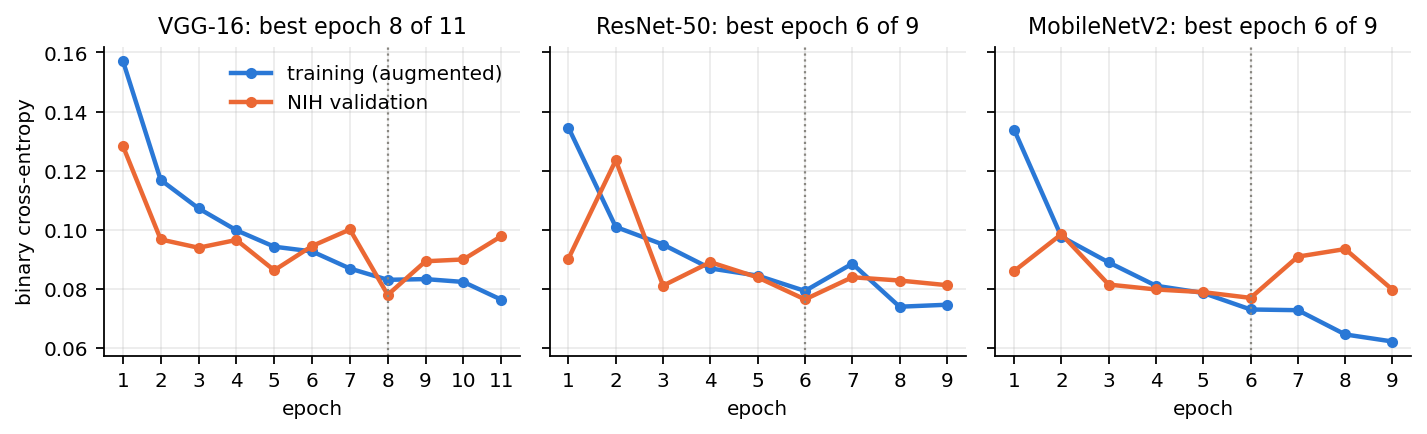
\includegraphics[width=\linewidth,height=0.66\textheight,keepaspectratio]{figures/training_curves.png}
\caption{Training and NIH validation loss per epoch; the dotted line marks the best epoch, whose weights are kept. Training loss is measured on augmented cells during the epoch.}
\end{figure}

All three stopped early, and their best NIH validation losses are within 0.002 of each other, so the three arms start the external tests equally well fitted to NIH. After the best epoch, validation loss rose for all three while training loss mostly kept falling: further epochs would only have fitted the training patients more closely.

\subsubsection*{RQ1: how large is the drop, and does the lighter architecture lose less?}

{\footnotesize
\begin{longtable}{@{}>{\raggedright\arraybackslash\hspace{0pt}}p{109.8pt}>{\raggedright\arraybackslash\hspace{0pt}}p{63.5pt}>{\raggedright\arraybackslash\hspace{0pt}}p{65.2pt}>{\raggedright\arraybackslash\hspace{0pt}}p{73.5pt}@{}}
\toprule
Test set, metric & VGG-16 & ResNet-50 & \mbox{MobileNetV2} \\
\midrule
\endhead
\bottomrule
\endfoot
\bottomrule
\caption{Values in \%, fixed threshold 0.5; drops in percentage points from the same model's NIH hold-out value. Intervals for every value and drop are in \href{https://github.com/noahtjonsk/malaria-cross-dataset/blob/main/outputs/tables/rq1_vgg16_s0.csv}{\texttt{rq1\_\allowbreak{}vgg16\_\allowbreak{}s0.\allowbreak{}csv}}, \href{https://github.com/noahtjonsk/malaria-cross-dataset/blob/main/outputs/tables/rq1_resnet50_s0.csv}{\texttt{rq1\_\allowbreak{}resnet50\_\allowbreak{}s0.\allowbreak{}csv}} and \href{https://github.com/noahtjonsk/malaria-cross-dataset/blob/main/outputs/tables/rq1_mobilenet_v2_s0.csv}{\texttt{rq1\_\allowbreak{}mobilenet\_\allowbreak{}v2\_\allowbreak{}s0.\allowbreak{}csv}}.}
\endlastfoot
NIH hold-out sensitivity & 98.2 (96.8 to 99.3) & 97.2 (95.6 to 98.5) & 97.1 (95.3 to 98.2) \\*
NIH hold-out specificity & 96.6 (94.7 to 97.9) & 98.4 (97.8 to 98.9) & 98.2 (97.5 to 98.8) \\*
site\_\allowbreak{}a sensitivity & 99.3 (drop \textminus{}1.1) & 79.3 (drop 17.9) & 83.7 (drop 13.4) \\*
site\_\allowbreak{}a specificity & 65.5 (drop 31.0) & 87.3 (drop 11.0) & 90.0 (drop 8.1) \\*
site\_\allowbreak{}a AUC & 97.2 (drop 2.5) & 92.0 (drop 7.6) & 94.5 (drop 5.1) \\*
site\_\allowbreak{}b sensitivity & 89.8 (drop 8.5) & 68.0 (drop 29.2) & 30.4 (drop 66.7) \\*
site\_\allowbreak{}b specificity & 95.0 (drop 1.5) & 98.1 (drop 0.2) & 99.1 (drop \textminus{}0.9) \\*
site\_\allowbreak{}b AUC & 97.5 (drop 2.2) & 96.4 (drop 3.2) & 93.0 (drop 6.6) \\*
MP-IDB \emph{P. falciparum} sensitivity & 57.4 (drop 40.9) & 52.6 (drop 44.6) & 28.6 (drop 68.5) \\*
MP-IDB other species sensitivity & 80.0 (drop 18.2) & 56.4 (drop 40.8) & 38.6 (drop 58.5) \\*
\end{longtable}}

\begin{figure}[H]
\centering
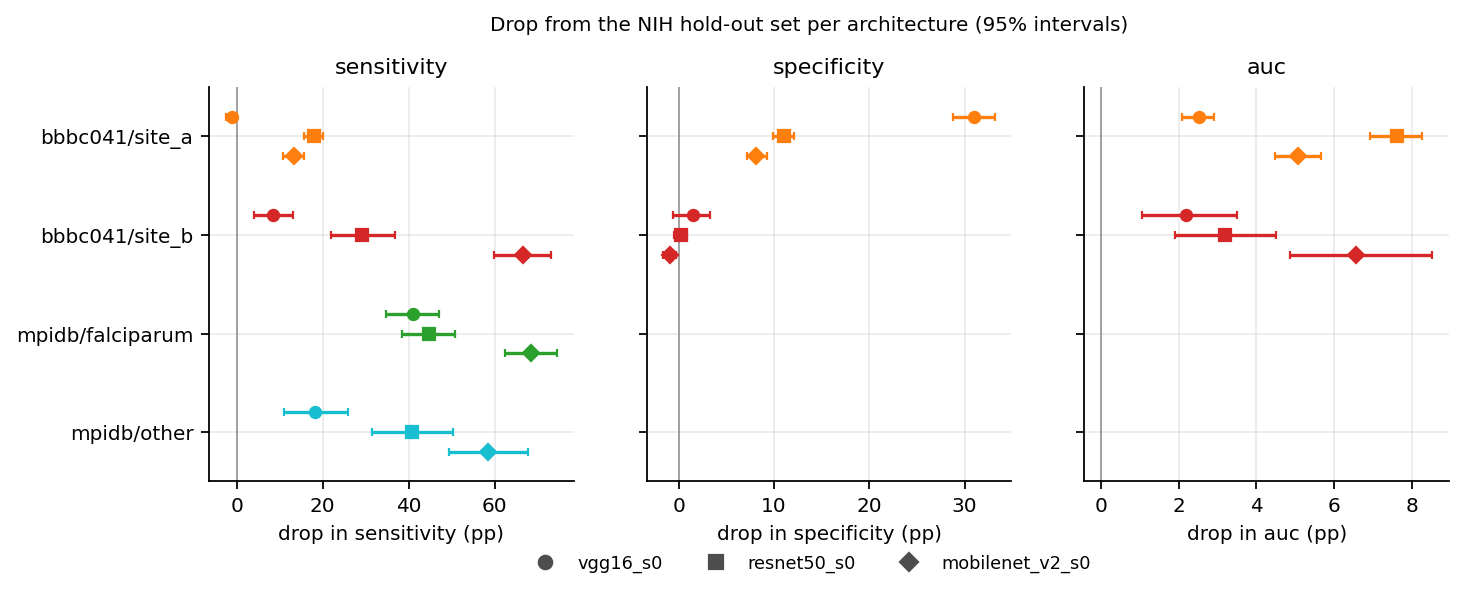
\includegraphics[width=\linewidth,height=0.66\textheight,keepaspectratio]{../../outputs/figures/R_compare_s0.png}
\caption{Drop from the NIH hold-out set per architecture, with 95\% intervals (\href{https://github.com/noahtjonsk/malaria-cross-dataset/blob/main/scripts/compare_models.py}{\texttt{compare\_\allowbreak{}models.\allowbreak{}py}}).}
\end{figure}

All three models do equally well on NIH (AUC 0.996 to 0.997), and all three lose on at least one metric on every external set, but they lose in different places. \mbox{MobileNetV2}, the lighter architecture, does not lose less. It loses the most sensitivity on site\_\allowbreak{}b and on both MP-IDB groups, by 17.7 to 58.2 points more than the heavier models, and every one of these differences stays clear of zero after the Bonferroni adjustment (for example 27.6 points more than VGG-16 on \emph{P. falciparum}, adjusted interval 20.5 to 34.4). On site\_\allowbreak{}a the order reverses: VGG-16 loses 31.0 points of specificity, 22.9 more than \mbox{MobileNetV2} (adjusted 19.8 to 25.9). VGG-16 has the smallest AUC drop on both BBBC041 sites. Of the 24 pairwise differences, 20 stay clear of zero after adjustment (\href{https://github.com/noahtjonsk/malaria-cross-dataset/blob/main/outputs/tables/rq1_compare_s0.csv}{\texttt{rq1\_\allowbreak{}compare\_\allowbreak{}s0.\allowbreak{}csv}}).

Much of the difference between the architectures comes from where their scores fall relative to the 0.5 threshold. VGG-16 calls 34\% of BBBC041 cells parasitised, against 14\% for ResNet-50 and 11\% for \mbox{MobileNetV2}. That is why VGG-16 keeps its sensitivity and loses specificity, while the other two do the opposite. AUC, which ignores the threshold, still favours VGG-16 on both sites. At the fixed threshold, the answer to RQ1's second part is no, with one caveat: part of the lighter model's loss is a shift of its scores toward \emph{uninfected} on the external sets.

\subsubsection*{Secondary measure: precision and F1}

{\footnotesize
\begin{longtable}{@{}>{\raggedright\arraybackslash\hspace{0pt}}p{89.8pt}>{\raggedright\arraybackslash\hspace{0pt}}p{43.9pt}>{\raggedright\arraybackslash\hspace{0pt}}p{48.9pt}>{\raggedright\arraybackslash\hspace{0pt}}p{51.7pt}>{\raggedright\arraybackslash\hspace{0pt}}p{65.8pt}@{}}
\toprule
Set & Measure & VGG-16 & ResNet-50 & \mbox{MobileNetV2} \\
\midrule
\endhead
\bottomrule
\endfoot
\bottomrule
\caption{Precision and F1 in \%, with 95\% intervals from resampling source images (NIH hold-out: patients), from \texttt{rq1\_\allowbreak{}f1\_\allowbreak{}<model>\_\allowbreak{}s0.\allowbreak{}csv}. Not computed on MP-IDB, which has no uninfected cells.}
\endlastfoot
NIH hold-out (49.2\% parasitised) & precision & 96.5 (90.6 to 98.4) & 98.3 (95.9 to 99.1) & 98.1 (95.2 to 99.0) \\*
 & F1 & 97.4 (94.1 to 98.5) & 97.7 (96.0 to 98.6) & 97.6 (95.5 to 98.4) \\*
site\_\allowbreak{}a (2.7\% parasitised) & precision & 7.4 (7.0 to 7.8) & 14.8 (13.6 to 16.2) & 18.9 (17.2 to 20.7) \\*
 & F1 & 13.8 (13.0 to 14.5) & 24.9 (23.1 to 26.9) & 30.8 (28.5 to 33.3) \\*
site\_\allowbreak{}b (5.1\% parasitised) & precision & 49.5 (44.2 to 55.4) & 66.2 (60.9 to 71.8) & 63.9 (55.7 to 72.3) \\*
 & F1 & 63.8 (59.0 to 68.7) & 67.1 (61.6 to 71.9) & 41.2 (33.9 to 47.7) \\*
\end{longtable}}

F1 is between 97.4 and 97.7\% on the NIH hold-out set for all three models and falls on BBBC041, most on site\_\allowbreak{}a, where precision is 7.4 to 18.9\%. At 2.7\% prevalence, VGG-16's site\_\allowbreak{}a specificity of 65.5\% still means 26,684 false alarms against 2,134 parasites found, 12.5 for every parasite. F1 puts VGG-16 last on site\_\allowbreak{}a although its site\_\allowbreak{}a AUC is the highest of the three. At this prevalence its false alarms outnumber the parasites, so its F1 depends mostly on how many cells it calls parasitised at the fixed threshold. For this reason F1 is reported next to sensitivity and specificity and does not replace them.

\subsubsection*{RQ3: species and life stages}

{\footnotesize
\begin{longtable}{@{}>{\raggedright\arraybackslash\hspace{0pt}}p{53.5pt}>{\raggedright\arraybackslash\hspace{0pt}}p{87.0pt}>{\raggedright\arraybackslash\hspace{0pt}}p{92.5pt}>{\raggedright\arraybackslash\hspace{0pt}}p{78.9pt}@{}}
\toprule
Model & \emph{P. falciparum} minus other species (pp, 95\% CI) & site\_\allowbreak{}a stage with most misses (share; miss rate) & site\_\allowbreak{}b stage with most misses (share; miss rate) \\
\midrule
\endhead
\bottomrule
\endfoot
\bottomrule
\caption{From \texttt{rq3\_\allowbreak{}<model>\_\allowbreak{}s0.\allowbreak{}csv}.}
\endlastfoot
VGG-16 & \textminus{}22.6 (\textminus{}31.7 to \textminus{}13.1) & ring (93\%; 4.0\%) & ring (71\%; 13.0\%) \\*
ResNet-50 & \textminus{}3.8 (\textminus{}14.9 to 7.7) & trophozoite (55\%; 16.5\%) & ring (64\%; 36.7\%) \\*
\mbox{MobileNetV2} & \textminus{}10.0 (\textminus{}21.0 to 0.7) & trophozoite (46\%; 11.0\%) & ring (52\%; 65.1\%) \\*
\end{longtable}}

Only VGG-16 shows a species gap larger than its interval, and it runs the opposite way to a species effect: \emph{P. falciparum}, the NIH species, is recognised less often. 1,230 of the 1,297 MP-IDB \emph{P. falciparum} parasites are rings. On BBBC041 site\_\allowbreak{}b, rings account for the largest share of misses for all three models (52 to 71\%). On site\_\allowbreak{}a, trophozoites (69\% of the parasites) account for the largest share of misses for ResNet-50 and \mbox{MobileNetV2}, while their miss rate stays below that of rings and gametocytes. Leaving out the 346 fallback crops lowers \emph{P. falciparum} sensitivity for all three models (to 53.2, 46.3 and 23.4\%) and widens the gap to the other species (\textminus{}27.4, \textminus{}10.4 and \textminus{}16.9 points). \mbox{MobileNetV2}'s gap then also lies outside its interval (\textminus{}28.3 to \textminus{}5.2), so for \mbox{MobileNetV2} the species result depends on these crops (\texttt{rq3\_\allowbreak{}<model>\_\allowbreak{}s0\_\allowbreak{}without\_\allowbreak{}fallback.\allowbreak{}csv}).

Rings are missed more often than trophozoites in five of the six model and site combinations. The exception is \mbox{MobileNetV2} on site\_\allowbreak{}b, which misses 65\% of rings and 80\% of trophozoites. Their size fits this: a ring is a chromatin dot of 1 to 2 \textmu{}m, a few pixels in a resized cell crop, while a mature trophozoite is 5 to 8 \textmu{}m \citep{hou2026}. Since most MP-IDB \emph{P. falciparum} parasites are rings, VGG-16's species gap may come from the stage mix and not from the species itself. The final analysis tests this by comparing ring sensitivity between the two MP-IDB groups, for each model and seed.

\subsubsection*{RQ2: background removal and colour matching}

{\footnotesize
\begin{longtable}{@{}>{\raggedright\arraybackslash\hspace{0pt}}p{64.2pt}>{\raggedright\arraybackslash\hspace{0pt}}p{54.3pt}>{\raggedleft\arraybackslash}p{23.3pt}>{\raggedleft\arraybackslash}p{53.6pt}>{\raggedleft\arraybackslash}p{41.9pt}>{\raggedleft\arraybackslash}p{50.6pt}@{}}
\toprule
Test set, metric & Model & Raw & Background removed & + Reinhard & + Histogram matching \\
\midrule
\endhead
\bottomrule
\endfoot
\bottomrule
\caption{Values in \%, for the four rows that carry the RQ2 findings; every external set and metric is in Appendix A, and the shares recovered and intervals in \texttt{rq2\_\allowbreak{}<model>\_\allowbreak{}s0.\allowbreak{}csv}.}
\endlastfoot
MP-IDB \emph{P. falciparum} sensitivity & VGG-16 & 57.4 & 71.9 & 66.4 & 99.5 \\*
 & ResNet-50 & 52.6 & 63.9 & 52.3 & 98.1 \\*
 & \mbox{MobileNetV2} & 28.6 & 27.2 & 32.9 & 95.4 \\*
site\_\allowbreak{}b sensitivity & VGG-16 & 89.8 & 90.8 & 89.8 & 100.0 \\*
 & ResNet-50 & 68.0 & 73.6 & 75.9 & 95.0 \\*
 & \mbox{MobileNetV2} & 30.4 & 36.6 & 47.2 & 80.5 \\*
site\_\allowbreak{}a specificity & VGG-16 & 65.5 & 53.6 & 74.9 & 5.9 \\*
 & ResNet-50 & 87.3 & 66.6 & 82.0 & 6.6 \\*
 & \mbox{MobileNetV2} & 90.0 & 78.9 & 96.3 & 44.4 \\*
site\_\allowbreak{}a AUC & VGG-16 & 97.2 & 96.6 & 85.6 & 91.6 \\*
 & ResNet-50 & 92.0 & 90.2 & 74.5 & 72.7 \\*
 & \mbox{MobileNetV2} & 94.5 & 89.6 & 84.1 & 88.5 \\*
\end{longtable}}

Removing the background raises MP-IDB \emph{P. falciparum} sensitivity for VGG-16 (recovering 36\% of its drop) and ResNet-50 (25\%), but not for \mbox{MobileNetV2}. It also raises site\_\allowbreak{}b sensitivity for all three models (by 1.0 to 6.2 points), while it lowers site\_\allowbreak{}a specificity for all three. Reinhard transfer raises site\_\allowbreak{}a specificity for VGG-16 and \mbox{MobileNetV2} but costs site\_\allowbreak{}a sensitivity, down to 15.9\% for \mbox{MobileNetV2}. Histogram matching pushes almost every cell to \emph{parasitised} for all three models: sensitivity is 80 to 100\% on every set, while specificity falls to 5.9 to 44.4\% on site\_\allowbreak{}a and 1.1 to 41.9\% on site\_\allowbreak{}b. Compared with the raw crops, no step raises AUC on either BBBC041 site for any model. Leaving out the 1,022 BBBC041 cells whose mask fell back to a neighbouring region changes no BBBC041 value by more than 2.2 points for any model (\texttt{rq2\_\allowbreak{}<model>\_\allowbreak{}s0\_\allowbreak{}without\_\allowbreak{}nearest.\allowbreak{}csv}).

At the fixed threshold, the colour steps mostly move the models' scores and, for all three architectures, do not improve how well the scores separate the classes. MP-IDB has no uninfected cells, so a higher sensitivity there cannot tell a better model from one that calls more cells parasitised: histogram matching ``recovers'' 85 to 110\% of the MP-IDB drops while it destroys specificity on BBBC041. RQ2's share recovered is read together with BBBC041 specificity and AUC for the same step (\S{}5.8).

\subsection{Methodological alternatives considered}

Most choices follow from one constraint: RQ2 can attribute a change in performance to a step only if the model and the test cells stay fixed in every other way.

{\footnotesize
\begin{longtable}{@{}>{\raggedright\arraybackslash\hspace{0pt}}p{70.9pt}>{\raggedright\arraybackslash\hspace{0pt}}p{78.0pt}>{\raggedright\arraybackslash\hspace{0pt}}p{65.5pt}>{\raggedright\arraybackslash\hspace{0pt}}p{97.6pt}@{}}
\toprule
Decision & Alternatives & Chosen & Why \\
\midrule
\endhead
\bottomrule
\endfoot
\bottomrule
\caption{Methodological alternatives considered and the choices made.}
\endlastfoot
Fine-tuning & frozen ImageNet features plus a new head \citep{rajaraman2018}; all layers trained & all layers trained & stain and cell texture are far from ImageNet photographs, so the early layers need to adapt too \\*
NIH split & random cell-level split \citep{zhao2020}; patient-grouped split & patient-grouped & a random split puts cells of one slide on both sides; \citet{hou2026} found per-cell accuracy 1.5 points higher than with a slide-disjoint split \\*
Hyperparameter search & grid search or Optuna per model; fixed values from the literature & fixed values & every architecture gets the same settings, so RQ1 compares architectures alone; fits a free Colab GPU \\
How to test the explanations (RQ2) & colour augmentation or retraining on target images; editing the test inputs & edit the test inputs & needs no target labels and keeps the model fixed, so each step's effect can be attributed to it; retraining would answer a different question \\
Background removal & rembg U\textsuperscript{2}-Net or IS-Net \citep{qin2020}; BiRefNet; Otsu on brightness & Otsu on brightness & median Dice 0.90 against the NIH hand-drawn outlines, against 0.03 for U\textsuperscript{2}-Net, which found no cell in 21\% of NIH crops; BiRefNet needs 31 s per crop on this laptop \\
Colour matching & HSV shift; Macenko \citep{macenko2009}; learned normalisation \citep{xu2025}; Reinhard and histogram matching & Reinhard and histogram matching & both are simple and fully specified, and the EDA showed they bring the Giemsa stain channels to NIH while an HSV shift moves them away; \citet{xu2025} found stain-vector methods beat Reinhard on malaria smears, so a Macenko step is a candidate extension \\
MP-IDB framing & shipped parasite close-ups; whole-cell crops & whole-cell crops & the close-ups cut off the cell edge, and the shipped crops mix masked and unmasked formats by species \\
Main metric & accuracy, F1 or AUC alone; sensitivity and specificity at 0.5 & sensitivity and specificity, with AUC and F1 as secondary & prevalence of 2.7 to 5.1\% on BBBC041; the two errors have different clinical costs \\*
Uncertainty & a single test score; cell-level bootstrap; image-level bootstrap & image-level (NIH: patient-level) bootstrap & cells of one image are not independent; gives intervals instead of point estimates \\*
\end{longtable}}

\subsection{Design decisions for the final analysis}

The baseline raised eight questions about how the final results will be computed and read. These are the decisions taken:

\begin{enumerate}
\item Fixed hyperparameters (Table 6) for all three arms, so that RQ1 compares architectures alone.
\item Three seeds per architecture for the final results, against one for the midterm baseline. The seeds give the run-to-run spread next to the bootstrap intervals.
\item A paired bootstrap with a Bonferroni correction for the RQ1 comparison: the 24 comparisons share one 5\% error budget, so each interval is widened to 99.8\%. At seed 0 the conclusion does not depend on the correction, since 20 of 24 differences stay clear with it.
\item Share recovered is left undefined unless the raw drop's 95\% interval lies above zero.
\item The RQ3 stage table shows the miss rate next to the share of misses, because the shares follow the stage counts.
\item The 346 fallback crops are kept, and RQ3 is also reported without them.
\item A sensitivity gain on MP-IDB counts as recovery only if AUC on BBBC041 does not fall for the same step, because MP-IDB cannot show whether the model simply calls more cells parasitised.
\item RQ1 reports the AUC drop next to the sensitivity and specificity drops as a threshold-free view, since the architectures differ mainly in where their scores fall relative to the 0.5 threshold.
\end{enumerate}

\section{Reproducibility}

All scripts live in the repository and are listed by the pipeline stage they implement (Figure 1).

{\small
\begin{longtable}{@{}>{\raggedright\arraybackslash\hspace{0pt}}p{29.4pt}>{\raggedright\arraybackslash\hspace{0pt}}p{158.1pt}>{\raggedright\arraybackslash\hspace{0pt}}p{136.5pt}@{}}
\toprule
Stage & Script & Purpose \\
\midrule
\endhead
\bottomrule
\endfoot
\bottomrule
\caption{Scripts by pipeline stage. The repository layout is in Appendix D.}
\endlastfoot
A & \texttt{malaria/\allowbreak{}paths.\allowbreak{}py}, \texttt{scripts/\allowbreak{}check\_\allowbreak{}nih\_\allowbreak{}overlap.\allowbreak{}py} & every dataset root and output folder; NIH-NLM release against cell\_\allowbreak{}images \\*
B & \texttt{scripts/\allowbreak{}build\_\allowbreak{}crops.\allowbreak{}py} (\texttt{malaria/\allowbreak{}manifests.\allowbreak{}py}, \texttt{crops.\allowbreak{}py}, \texttt{background.\allowbreak{}py}) & manifests and crops; MP-IDB host-cell framing \\*
C & \texttt{malaria/\allowbreak{}splits.\allowbreak{}py} & patient-grouped split, pinned in \texttt{nih\_\allowbreak{}split.\allowbreak{}csv}; leakage check \\
D & \texttt{scripts/\allowbreak{}compute\_\allowbreak{}stats.\allowbreak{}py}, \texttt{compute\_\allowbreak{}colour\_\allowbreak{}stats.\allowbreak{}py}, \texttt{validate\_\allowbreak{}background.\allowbreak{}py}; \texttt{notebooks/\allowbreak{}03\_\allowbreak{}eda\_\allowbreak{}short.\allowbreak{}ipynb} & per-cell statistics on tissue pixels; background-method scores; the EDA \\
E & \texttt{scripts/\allowbreak{}train.\allowbreak{}py} (\texttt{malaria/\allowbreak{}models.\allowbreak{}py}, \texttt{data.\allowbreak{}py}); \texttt{scripts/\allowbreak{}pack\_\allowbreak{}for\_\allowbreak{}colab.\allowbreak{}py}; \texttt{notebooks/\allowbreak{}10\_\allowbreak{}train\_\allowbreak{}colab.\allowbreak{}ipynb} & fine-tuning on NIH; data archives for Colab; the Colab run \\
F & \texttt{scripts/\allowbreak{}build\_\allowbreak{}masked\_\allowbreak{}crops.\allowbreak{}py}, \texttt{build\_\allowbreak{}colour\_\allowbreak{}crops.\allowbreak{}py} (\texttt{malaria/\allowbreak{}colour.\allowbreak{}py}) & background removal; Reinhard and histogram matching \\
G & \texttt{scripts/\allowbreak{}evaluate.\allowbreak{}py} & frozen inference, one prediction file per variant and set, with a \texttt{run.\allowbreak{}json} record \\
H & \texttt{scripts/\allowbreak{}summarise\_\allowbreak{}results.\allowbreak{}py}, \texttt{compare\_\allowbreak{}models.\allowbreak{}py} (\texttt{malaria/\allowbreak{}metrics.\allowbreak{}py}, \texttt{results.\allowbreak{}py}) & RQ1, F1, RQ2 and RQ3 tables per model; paired differences in drop between models \\*
all & \texttt{scripts/\allowbreak{}make\_\allowbreak{}mo\_\allowbreak{}figures.\allowbreak{}py}, \texttt{build\_\allowbreak{}mo\_\allowbreak{}latex.\allowbreak{}py}, \texttt{build\_\allowbreak{}mo\_\allowbreak{}pdf.\allowbreak{}py} & the figures; this document as LaTeX and PDF; the ELSA report as PDF \\*
\end{longtable}}

To reproduce the work, download the three datasets from the sources in \S{}2.1 into the project root, then run from the repository root:

\begin{Verbatim}[fontsize=\fontsize{6.5}{8}\selectfont,frame=none]
pip install -r requirements.txt
python -m malaria.metrics                      # metric self-test
python scripts/train.py --arch vgg16 --smoke --no-pretrained   # CPU smoke check
python scripts/build_crops.py                  # manifests and crops (A, B, C)
python scripts/build_crops.py --mpidb-wholecell
python scripts/compute_stats.py --workers 6    # EDA statistics (D)
python scripts/compute_stats.py --manifest mpidb_wholecell_cells.csv
python scripts/build_masked_crops.py --method otsu-gray --datasets bbbc041 mpidb_wholecell   # F1
python scripts/build_colour_crops.py           # F2
python scripts/pack_for_colab.py               # code.zip, data_raw.zip, data_rq2.zip
# on Colab, through notebooks/10_train_colab.ipynb, for each of vgg16, resnet50, mobilenet_v2:
python scripts/train.py --arch vgg16 --seed 0 --resume
python scripts/evaluate.py --checkpoint models/vgg16_s0.pt --variants raw masked reinhard histmatch
python scripts/summarise_results.py --model vgg16_s0
# then once:
python scripts/compare_models.py               # RQ1: paired differences in drop
\end{Verbatim}

The full run order, including the EDA-only steps, is in \href{https://github.com/noahtjonsk/malaria-cross-dataset/blob/main/README.md}{\texttt{README.\allowbreak{}md}}. Seeds are fixed for the split (42), the colour reference sample (0), the bootstrap (0) and each training run (\texttt{--seed}).

The code, the pinned split, the manifests' build logic and every summary table are public in the repository. The images are not: anyone reproducing the work downloads the three datasets from the sources in \S{}2.1 and places them in the project root. Training needs a GPU (a free Colab T4 is enough: about three minutes per epoch for VGG-16, under two for the other two models); everything else runs on a CPU. Following \citet{dicosmo2026}, the repository will be archived with a persistent identifier at the end of the project.

\nocite{aiact2024,mdr2017}
\printbibliography[heading=ctbib,title=References]

\appendix
\setcounter{table}{0}\renewcommand{\thetable}{A\arabic{table}}

\clearpage
\section{Full RQ2 table}

{\footnotesize
\begin{longtable}{@{}>{\raggedright\arraybackslash\hspace{0pt}}p{64.2pt}>{\raggedright\arraybackslash\hspace{0pt}}p{54.3pt}>{\raggedleft\arraybackslash}p{23.3pt}>{\raggedleft\arraybackslash}p{53.6pt}>{\raggedleft\arraybackslash}p{41.9pt}>{\raggedleft\arraybackslash}p{50.6pt}@{}}
\toprule
Test set, metric & Model & Raw & Background removed & + Reinhard & + Histogram matching \\
\midrule
\endhead
\bottomrule
\endfoot
\bottomrule
\caption{Every external set and metric, in \%, seed 0. Per-model figures: \href{https://github.com/noahtjonsk/malaria-cross-dataset/blob/main/outputs/figures/R_vgg16_s0.png}{\texttt{R\_\allowbreak{}vgg16\_\allowbreak{}s0.\allowbreak{}png}}, \href{https://github.com/noahtjonsk/malaria-cross-dataset/blob/main/outputs/figures/R_resnet50_s0.png}{\texttt{R\_\allowbreak{}resnet50\_\allowbreak{}s0.\allowbreak{}png}}, \href{https://github.com/noahtjonsk/malaria-cross-dataset/blob/main/outputs/figures/R_mobilenet_v2_s0.png}{\texttt{R\_\allowbreak{}mobilenet\_\allowbreak{}v2\_\allowbreak{}s0.\allowbreak{}png}}.}
\endlastfoot
site\_\allowbreak{}a sensitivity & VGG-16 & 99.3 & 99.4 & 80.5 & 99.8 \\*
 & ResNet-50 & 79.3 & 92.6 & 42.8 & 98.4 \\*
 & \mbox{MobileNetV2} & 83.7 & 84.3 & 15.9 & 96.6 \\
site\_\allowbreak{}b sensitivity & VGG-16 & 89.8 & 90.8 & 89.8 & 100.0 \\
 & ResNet-50 & 68.0 & 73.6 & 75.9 & 95.0 \\
 & \mbox{MobileNetV2} & 30.4 & 36.6 & 47.2 & 80.5 \\
MP-IDB \emph{P. falciparum} sensitivity & VGG-16 & 57.4 & 71.9 & 66.4 & 99.5 \\
 & ResNet-50 & 52.6 & 63.9 & 52.3 & 98.1 \\
 & \mbox{MobileNetV2} & 28.6 & 27.2 & 32.9 & 95.4 \\
MP-IDB other species sensitivity & VGG-16 & 80.0 & 82.9 & 70.0 & 100.0 \\
 & ResNet-50 & 56.4 & 67.9 & 42.1 & 99.3 \\
 & \mbox{MobileNetV2} & 38.6 & 37.9 & 28.6 & 88.6 \\
site\_\allowbreak{}a specificity & VGG-16 & 65.5 & 53.6 & 74.9 & 5.9 \\
 & ResNet-50 & 87.3 & 66.6 & 82.0 & 6.6 \\
 & \mbox{MobileNetV2} & 90.0 & 78.9 & 96.3 & 44.4 \\
site\_\allowbreak{}b specificity & VGG-16 & 95.0 & 86.2 & 80.3 & 1.1 \\
 & ResNet-50 & 98.1 & 98.3 & 89.8 & 15.0 \\
 & \mbox{MobileNetV2} & 99.1 & 97.2 & 98.1 & 41.9 \\
site\_\allowbreak{}a AUC & VGG-16 & 97.2 & 96.6 & 85.6 & 91.6 \\
 & ResNet-50 & 92.0 & 90.2 & 74.5 & 72.7 \\
 & \mbox{MobileNetV2} & 94.5 & 89.6 & 84.1 & 88.5 \\
site\_\allowbreak{}b AUC & VGG-16 & 97.5 & 95.8 & 93.7 & 73.0 \\
 & ResNet-50 & 96.4 & 96.1 & 91.6 & 72.5 \\*
 & \mbox{MobileNetV2} & 93.0 & 87.2 & 87.6 & 69.4 \\*
\end{longtable}}

\clearpage
\section{Model information sheet}

{\small
\begin{longtable}{@{}>{\raggedright\arraybackslash\hspace{0pt}}p{69.8pt}>{\raggedright\arraybackslash\hspace{0pt}}p{266.2pt}@{}}
\toprule
Field & Value \\
\midrule
\endhead
\bottomrule
\endfoot
\bottomrule
\endlastfoot
Task & Binary classification of a single red-cell image as parasitised or uninfected \\*
Input & One RGB cell crop, padded to a square with black, 224 $\times$ 224, ImageNet-normalised \\*
Output & A logit; the cell is called parasitised when the probability is at least 0.5 \\
Training population & 19,203 NIH cells from 140 patients, one hospital in Chittagong, \emph{P. falciparum} only, about 50\% parasitised \\
External evaluation & BBBC041 site\_\allowbreak{}a and site\_\allowbreak{}b (\emph{P. vivax}, 2.7 to 5.1\% parasitised) and MP-IDB (four species, parasitised cells only), without fine-tuning \\
Intended use & Academic research into why CNN malaria classifiers lose performance across datasets \\
Out-of-scope use & Diagnosis or screening of patients, or any clinical decision; the model has no clinical validation \\
Known limitations & Single training site and species; no demographic variables; one seed at the midterm; MP-IDB has no uninfected cells, so specificity is measured on BBBC041 only \\*
Failure modes seen so far & Large loss of sensitivity on MP-IDB \emph{P. falciparum} for every architecture; VGG-16 raises many false alarms on BBBC041 site\_\allowbreak{}a, while ResNet-50 and \mbox{MobileNetV2} miss more parasites; \mbox{MobileNetV2} misses most site\_\allowbreak{}b parasites; colour matching shifts scores toward \emph{parasitised} (\S{}5.6) \\*
\end{longtable}}
\addtocounter{table}{-1}

\clearpage
\section{Continuous-analysis checks}

{\small
\begin{longtable}{@{}>{\raggedright\arraybackslash\hspace{0pt}}p{241.1pt}>{\raggedright\arraybackslash\hspace{0pt}}p{94.9pt}@{}}
\toprule
Check & Where \\
\midrule
\endhead
\bottomrule
\endfoot
\bottomrule
\endlastfoot
NIH split sizes equal the pinned 19,203 / 4,178 / 4,177; every NIH cell has a split & \texttt{data.\allowbreak{}nih\_\allowbreak{}cells} \\*
No patient in two splits; train and validation patients disjoint & \texttt{splits.\allowbreak{}check\_\allowbreak{}no\_\allowbreak{}patient\_\allowbreak{}leakage}, \texttt{train.\allowbreak{}py} \\*
Every parameter trainable (the weights are unfrozen) & \texttt{models.\allowbreak{}check\_\allowbreak{}all\_\allowbreak{}trainable} \\
Unlabelled or excluded rows never reach a model & \texttt{data.\allowbreak{}CellDataset}, \texttt{data.\allowbreak{}test\_\allowbreak{}cells} \\
Reframing keeps every MP-IDB parasite, stage label and cell ID & \texttt{build\_\allowbreak{}crops.\allowbreak{}py --mpidb-wholecell} \\
Colour-matched manifests keep the row count of their input & \texttt{build\_\allowbreak{}colour\_\allowbreak{}crops.\allowbreak{}py} \\
Metrics on a perfect predictor: sensitivity, specificity, precision and F1 are 1, drop 0; the weighted AUC and F1 equal scikit-learn's; a set with one class has no precision or F1 & \texttt{python -m malaria.\allowbreak{}metrics} \\
A prediction file is reused only if its checkpoint, manifests, crop contents and row count still match; files are written atomically & \texttt{evaluate.\allowbreak{}py}, \texttt{results.\allowbreak{}load} \\
Models are compared only if they were scored on the same manifests, crop contents and cells & \texttt{compare\_\allowbreak{}models.\allowbreak{}check\_\allowbreak{}same\_\allowbreak{}inputs} \\
RQ2 variants hold the same cells & \texttt{summarise\_\allowbreak{}results.\allowbreak{}check\_\allowbreak{}same\_\allowbreak{}cells} \\
The fallback check removes exactly the 346 MP-IDB cells listed in the framing table & \texttt{summarise\_\allowbreak{}results.\allowbreak{}without\_\allowbreak{}fallback} \\*
The training curves' best epoch and loss match the training log & \texttt{make\_\allowbreak{}mo\_\allowbreak{}figures.\allowbreak{}training\_\allowbreak{}curves} \\*
\end{longtable}}
\addtocounter{table}{-1}

\clearpage
\section{Repository organisation}

\begin{Verbatim}[fontsize=\fontsize{6.5}{8}\selectfont,frame=none]
malaria-cross-dataset/
|-- README.md                    # run order and where every crop is saved
|-- requirements.txt             # pinned Python packages
|-- LiteratureReview_NoahTjonSienKie.pdf   # D2
|
|-- malaria/                     # the package every script imports
|   |-- paths.py                 # all dataset roots, output folders and measured constants
|   |-- crops.py                 # Stage B: square_padded_box cropping rule
|   |-- manifests.py             # Stage B: one manifest schema, builders per dataset
|   |-- splits.py                # Stage C: patient-grouped split, leakage check
|   |-- imagestats.py            # Stage D: per-cell features on tissue pixels, separation
|   |-- background.py            # Stages B/F: Otsu masks, host-cell framing, Dice
|   |-- colour.py                # Stage F: Reinhard, histogram matching, stain channels
|   |-- data.py                  # Stage E: nih_cells, test_cells, CellDataset
|   |-- models.py                # Stage E: build_model, check_all_trainable
|   |-- metrics.py               # Stage H: rates, F1, drop, share recovered, bootstrap
|   |-- results.py               # Stage H: reads prediction files back as the reported sets
|   |-- provenance.py            # code commit, manifest hashes and crop digests of every run
|   `-- plots.py                 # figure helpers
|
|-- scripts/
|   |-- build_crops.py           # Stage B: manifests and crops
|   |-- check_nih_overlap.py     # Stage A: NIH-NLM release vs cell_images
|   |-- compute_stats.py         # Stage D: per-cell statistics
|   |-- compute_colour_stats.py  # Stage D: colour-space statistics
|   |-- validate_background.py   # Stage D: scores background-removal methods
|   |-- build_masked_crops.py    # Stage F1: background removal
|   |-- build_colour_crops.py    # Stage F2: Reinhard and histogram matching
|   |-- pack_for_colab.py        # Stage E: data archives for Colab
|   |-- train.py                 # Stage E: fine-tuning
|   |-- evaluate.py              # Stage G: frozen inference, per-cell predictions
|   |-- summarise_results.py     # Stage H: RQ1/F1/RQ2/RQ3 tables and figure, per model
|   |-- compare_models.py        # Stage H: RQ1 paired differences in drop between models
|   |-- make_mo_figures.py       # figures for this document
|   |-- build_mo_latex.py        # this document as LaTeX and PDF
|   |-- build_mo_pdf.py          # the ELSA report as PDF
|   `-- make_notebook.py         # generates notebooks/01_eda.ipynb
|
|-- notebooks/
|   |-- 01_eda.ipynb             # full EDA record (generated)
|   |-- 03_eda_short.ipynb       # short EDA, the version presented
|   `-- 10_train_colab.ipynb     # Stages E and G on a Colab GPU
|
|-- data/
|   |-- manifests/
|   |   |-- nih_split.csv        # tracked: pins the train/val/hold-out rows
|   |   |-- mpidb_stage_audit.csv  # tracked: source of every MP-IDB stage label
|   |   `-- *_cells.csv          # gitignored: rebuilt by build_crops.py
|   `-- crops/                   # gitignored: about 87k PNGs, rebuilt by the build scripts
|
|-- outputs/
|   |-- figures/                 # EDA and results figures
|   |-- tables/                  # summary tables (rq1/rq2/rq3, F1, colour reference, overlap)
|   `-- predictions/             # gitignored: per-cell predictions (kept on Drive)
|
|-- models/                      # gitignored: trained weights (0.5 GB per VGG-16)
|
`-- docs/
    |-- methodology_overview_v3.md   # this document (D3), and its PDF
    |-- methodology_overview.md  # the earlier Markdown version
    |-- elsa_report.md           # D5: final checklist, mitigations, panel reflections
    |-- elsa_checklist.md        # the earlier working checklist
    `-- methodology/             # LaTeX source (mo_v3.tex, refs.bib) and figures of this document
\end{Verbatim}

The four source datasets (\texttt{cell\_\allowbreak{}images\_\allowbreak{}NIH/\allowbreak{}}, \texttt{malaria\_\allowbreak{}BBBC041/\allowbreak{}}, \texttt{MP-IDB-…/\allowbreak{}}, \texttt{NIH-NLM-ThinBloodSmearsPf/\allowbreak{}}) sit in the project root and are gitignored. Images and crops are never committed, because of their size and because BBBC041's licence requires derived data to be shared under the same terms.

\end{document}
